%% 02-covariates.tex — Glasgow Day 2 (afternoon): Covariates in DiD
%% Scott Cunningham, University of Glasgow, May 19, 2026
%%
%% Compile: pdflatex 02-covariates.tex
%% Style:   remix.sty (in same directory)
%%
%% Pedagogical structure: problem -> narrative -> picture -> codeblock -> intuition -> technical
%% Source material:
%%   /Users/scunning/Causal-Inference-2/Slides/Tex/02-Covariates.tex (heavy copy)
%%   /Users/scunning/the-remix-tour/glasgow/decks/code/IPW-Demo/ (existing pscore-critique sim)
%%   /Users/scunning/Library/CloudStorage/.../readings/SantAnna_DiD_CompositionalChanges_text.md
%%
%% NEW pedagogical block: the "can't I just control for the pscore?" trap
%%   (Lesson 4). Built fresh from the IPW-Demo + glasgow_content_map.md
%%   notes. Placed BEFORE DR so that DR's value is properly motivated.

\documentclass[aspectratio=169,11pt]{beamer}
\usepackage{remix}

\usepackage{tikz}
\usetikzlibrary{positioning,arrows.meta,calc,shapes.geometric,fit,backgrounds}
\usepackage{listings}
\usepackage{xcolor}
\usepackage{booktabs}
\usepackage{colortbl}

\lstset{
  basicstyle=\ttfamily\footnotesize,
  keywordstyle=\color{accentdark}\bfseries,
  commentstyle=\color{warmgray}\itshape,
  stringstyle=\color{ocean},
  backgroundcolor=\color{lightbg},
  frame=single,
  framesep=4pt,
  rulecolor=\color{warmgray!40},
  columns=fullflexible,
  showstringspaces=false,
  breaklines=true,
  numbers=none,
  xleftmargin=0.4em,
  xrightmargin=0.4em,
}

\renewcommand{\remixfooter}{University of Glasgow\,\textperiodcentered\,Adam Smith Business School\,\textperiodcentered\,May 2026}

\begin{document}

%% =====================================================================
%%                                ACT I
%% =====================================================================

%% ---------- Slide 1: TITLE ----------
\remixtitleframe
  {Covariates in DiD}
  {Day 2 of 5: Afternoon}
  {Scott Cunningham \textperiodcentered\ Baylor University}
  {University of Glasgow \textperiodcentered\ May 19, 2026}

%% ---------- Slide 2: Where we are ----------
\begin{frame}{The PT-violation problem, take two}
\vspace{0.5em}
\begin{itemize}
  \item This morning: a \highlight{third group} that shares the differential trend.
  \item But often, you don't have a clean placebo group.
  \item This afternoon: \highlight{condition on covariates that absorb the differential trend.}
\end{itemize}
\vspace{0.6em}
\begin{block}{Today's three estimators, and one false friend}
\small
\textbf{OR} (outcome regression) \;\; \textbf{IPW} (inverse propensity weighting) \;\; \textbf{DR} (doubly robust) \\[0.3em]
And: ``\textit{can't I just control for the propensity score in a regression?}'' \\
\highlight{That's the false friend.} We'll see why before DR.
\end{block}
\end{frame}

%% ---------- Slide 3: The applied problem ----------
\begin{frame}{The applied problem}
\vspace{0.5em}
\begin{itemize}
  \item Your treated states differ from your controls on observables --- baseline income, demographics, industry mix, education.
  \item If $Y(0)$ trends differ across these dimensions, unconditional PT is implausible.
  \item But maybe \textit{within} strata of $X$, PT holds:
\end{itemize}
\vspace{0.4em}
\begin{center}
\small
$\mathbb{E}[\Delta Y(0) \mid D=1, X] \;=\; \mathbb{E}[\Delta Y(0) \mid D=0, X]$
\end{center}
\vspace{0.5em}
\begin{itemize}
  \item This is \highlight{conditional parallel trends}. The escape valve for designs without a placebo group.
  \item Three estimators target this. They differ in \textit{which side} of the conditioning they model.
\end{itemize}
\end{frame}

%% ---------- Slide 4: Today's six beats ----------
\begin{frame}{This afternoon, six beats}
\vspace{0.3em}
\begin{enumerate}\small
  \item Outcome regression (Heckman-Ichimura-Todd, 1997) --- the bias OLS-with-controls actually identifies, plus the conditional-PT assumption that anchors the rest of the afternoon
  \item Inverse propensity weighting (Abadie 2005)
  \item Doubly robust DiD (Sant'Anna \& Zhao 2020)
  \item Hidden linearity bias --- TWFE-with-controls fully exposed (Caetano \& Callaway 2024)
  \item Choosing \& checking $X$ --- the practical close
\end{enumerate}
\vspace{0.4em}
\begin{center}
\small\color{warmgray}\itshape
We lead with the bias of OLS. \;\;Each fix below removes one piece of that bias.
\end{center}
\end{frame}

%% =====================================================================
%%                                LESSON 1
%% =====================================================================
\remixsection{1.\ Outcome Regression \\[0.3em] {\normalsize\normalfont What OLS-with-controls gives you --- and what it doesn't}}

%% ---------- L1-F0a: Conditional PT — the identifying assumption ----------
%% ---------- L1-F1: the assumption ----------
\begin{frame}{Conditional parallel trends, formally}
\vspace{0.4em}
\begin{block}{The new identifying assumption}
\small
\centering
$\mathbb{E}[\Delta Y(0) \mid D{=}1, X] \;=\; \mathbb{E}[\Delta Y(0) \mid D{=}0, X]$
\end{block}
\vspace{0.5em}
\begin{itemize}\small
  \item Within strata of $X$, the untreated trend is the same for treated and control.
  \item Equivalently: \textit{any} differential trend across treated and control is fully explained by their differences in $X$.
  \item Trade-off: weaker than unconditional PT (good), but you have to pick the right $X$ (hard).
  \item Two ways to use $X$: model the outcome side ($\mu(X)$), or model the treatment side ($p(X)$). Each is one of our estimators.
\end{itemize}
\end{frame}

%% ---------- L1-F0b: A note on history of thought ----------
\begin{frame}{A note on history of thought}
\footnotesize
\textbf{The first articulation of any parallel-trends-type assumption} in the DiD literature is:
\begin{block}{Heckman, Ichimura \& Todd (1997), \textit{Review of Economic Studies}}
\small
``Matching as an econometric evaluation estimator: evidence from evaluating a job training programme.''
\end{block}

\vspace{0.4em}
\textbf{The irony.} What HIT wrote down was the \highlight{\textit{conditional}} PT assumption ---
$\mathbb{E}[\Delta Y(0) \mid D{=}1, X] = \mathbb{E}[\Delta Y(0) \mid D{=}0, X]$.

\vspace{0.5em}
\textbf{Unconditional PT came later.} \;The morning's version --- $\mathbb{E}[\Delta Y(0) \mid D{=}1] = \mathbb{E}[\Delta Y(0) \mid D{=}0]$ --- is the special case of HIT's assumption with no $X$.

\vspace{0.5em}
\meta{The first PTA written down was the conditional one. \;The unconditional one is what the textbook taught next.}
\end{frame}

%% ---------- L2-F2: TWFE with controls ----------
\begin{frame}{The TWFE-with-controls regression --- and the three assumptions it hides}
\vspace{0.4em}
\[
Y_{it} \;=\; \alpha_i \;+\; \gamma_t \;+\; \delta\, (D_i {\times} \text{post}_t) \;+\; \beta\, X_{it} \;+\; \varepsilon_{it}
\]
\vspace{0.2em}
\begin{center}
\textbf{``Sure! If you're willing to impose three more assumptions.''}
\end{center}

\vspace{0.8em}
\begin{center}
\footnotesize
$\underbrace{\;\;\delta \text{ doesn't depend on } X\;\;}_{\textstyle\color{accent}\downarrow\;\;\textbf{Bias}_{\text{HTE}}}
\;\;\;
\underbrace{\;\;X \text{ has parallel trends across groups}\;\;}_{\textstyle\color{accent}\downarrow\;\;\textbf{Bias}_{\Delta X}}
\;\;\;
\underbrace{\;\;X \text{ is time-invariant}\;\;}_{\textstyle\color{accent}\downarrow\;\;\textbf{Bias}_{\text{FE}}}$
\end{center}

\vspace{0.6em}
\begin{itemize}\setlength\itemsep{1pt}\footnotesize
  \item $\textbf{Bias}_{\textbf{HTE}}$. \;If $\delta(X)$ varies with $X$, TWFE fits one $\delta$. \;\textit{Y(1) problem.}
  \item $\textbf{Bias}_{\boldsymbol{\Delta X}}$. \;If $X$ is imbalanced and drives $Y(0)$'s trend, PTA fails. \;\textit{Y(0) problem.}
  \item $\textbf{Bias}_{\textbf{FE}}$. \;You needed $X$ to defend \textit{conditional} PT --- but $\alpha_i$ demeans time-invariant $X$ to zero, silently restoring \textit{unconditional} PT. \;Fix: $\text{Post}\times X_{i,0}$ (pre-period $X$; \textit{next slide}).
\end{itemize}
\end{frame}

%% ---------- L2-F0z: Why we need X(1) = X(0) — derivation showing the residual ----------
\begin{frame}{Why we need $X(1) = X(0)$: the cross-term decomposition}
\scriptsize
\textbf{TWFE cell means} (CPT + no anticipation), with $X_{Dt}\equiv E[X\mid D, t]$:
\[
\begin{array}{rl@{\qquad}rl}
E[Y_1\mid D{=}1] &= \alpha_1 + \alpha_2 + \alpha_3 + \delta + \beta X_{11} &
E[Y_0\mid D{=}1] &= \alpha_1 + \alpha_3 + \beta X_{10} \\[2pt]
E[Y_1\mid D{=}0] &= \alpha_1 + \alpha_2 + \beta X_{01} &
E[Y_0\mid D{=}0] &= \alpha_1 + \beta X_{00}
\end{array}
\]

\textbf{Take the DiD.} \;The $\alpha$'s cancel; what's left is:
\[
\delta^{DD} \;=\; \delta \;+\; \beta\,\big[\,(X_{11} - X_{10}) \;-\; (X_{01} - X_{00})\,\big]
\]

\textbf{Switching equation for $X$:} \;controls are never treated, so $X_{00} = X_{01}$ (diff $=0$); for treated, $X_{10} = E[X(0)|D{=}1]$ and $X_{11} = E[X(1)|D{=}1]$. \;Substitute:
\[
\delta^{DD} \;=\; \delta \;+\; \beta\,\underbrace{E\big[X(1) - X(0)\mid D{=}1\big]}_{\text{treatment effect of }D\text{ on }X}
\]

\textbf{The cross-term cancels iff $X(1) = X(0)$.} \;Otherwise the residual is $\beta$ times the \highlight{treatment effect on $X$} (Angrist--Pischke bad control).

\textbf{Two fixes:} \;assume $X_i(1) = X_i(0) = X_i$ (demographics); or use $X_{i,0}$ everywhere (pre-period $X$ is mechanically $X(0)$ by no-anticipation).
\end{frame}

%% =========================================================================
%%   Bias_HTE — heterogeneous treatment effects in X. About Y(1).
%% =========================================================================

%% ---------- L2-HTE-1: Bias_HTE — intuition and PO ----------
\begin{frame}{$\text{Bias}_{\text{HTE}}$: when treatment effects depend on $X$}
\footnotesize
\textbf{In plain English.} \;Treatment doesn't work the same for everyone. \;Younger workers gain more from training than older ones; men gain more than women. \;That heterogeneity lives in $Y(1)$.

\vspace{0.5em}
\textbf{In potential outcomes:}
\[
\delta(X) \;\equiv\; \mathbb{E}[Y(1) - Y(0) \mid X,\,D{=}1] \;\;\text{is a \textit{function} of } X.
\]
The true ATT averages $\delta(X)$ over the treated $X$-distribution:
\[
\text{ATT} \;=\; \mathbb{E}\big[\delta(X) \mid D{=}1\big].
\]

\textbf{What TWFE-additive-$X$ fits:} \;one scalar $\hat{\delta}$. \;A weighted average of $\delta(X)$ whose weights are determined by OLS mechanics, \textit{not} the treated $X$-distribution.

\vspace{0.4em}
\highlight{Note: PTA on $Y(0)$ can hold perfectly --- $\text{Bias}_{\text{HTE}}$ is a $Y(1)$ problem, not a $Y(0)$ problem.}
\end{frame}

%% ---------- L2-HTE-2: Bias_HTE — Stata, building Y(0) and Y(1) by hand ----------
\begin{frame}[fragile]{$\text{Bias}_{\text{HTE}}$ in Stata}
\footnotesize
\begin{lstlisting}[language={[ANSI]C},basicstyle=\ttfamily\scriptsize]
* Y(0): same for everyone of a given age
gen y0 = 1000 + 5*age + rnormal(0, 10)

* Y(1) = Y(0) + delta(X). Treatment effect grows with age.
gen y1 = y0 + 200 + 50*age           // delta(age) = 200 + 50*age
gen delta = y1 - y0                  // varies by age

* True ATT (over treated X-distribution)
summarize delta if treat == 1
\end{lstlisting}

\vspace{0.4em}
\begin{itemize}\setlength\itemsep{2pt}
  \item Look at $\delta$: \;\;$\delta_i = 200 + 50\,\text{age}_i$. \;Not a constant.
  \item TWFE-additive-$X$ on the panel returns one $\hat{\delta}$. \;That number is a weighted average of $\delta$ that doesn't match $\mathbb{E}[\delta \mid D=1]$.
\end{itemize}
\end{frame}

%% =========================================================================
%%   Bias_DeltaX — Y(0) trend depends on X with X imbalance. About Y(0).
%% =========================================================================

%% ---------- L2-DX-1: Bias_DeltaX — lead with the RCT intuition ----------
\begin{frame}{$\text{Bias}_{\Delta X}$: imbalance in $X$ that drives $Y(0)$}
\footnotesize
\textbf{The RCT analogy.} \;Earnings $Y$ depends on a million $X$s (gender, age, education, neighborhood, ...). \;Randomization \textit{balances} those $X$s across treatment and control, so the $X \to Y$ channels cancel.

\vspace{0.5em}
\textbf{DiD without randomization.} \;If treated and control look different on $X$, and those $X$s drive $Y(0)$'s trend, then the group-level $Y(0)$ trends differ --- and PTA on $Y(0)$ fails.

\vspace{0.5em}
\textbf{A simple example.} \;Earnings change: \;men $+\$2$, women $+\$1$. \;Same for everyone (no treatment effect).
\begin{itemize}\setlength\itemsep{2pt}
  \item Treated 75\% male, control 25\% male:
  \item $\;\;\mathbb{E}[\Delta Y(0) \mid D{=}1] = 0.75(2) + 0.25(1) = 1.75$
  \item $\;\;\mathbb{E}[\Delta Y(0) \mid D{=}0] = 0.25(2) + 0.75(1) = 1.25$
  \item Naive DiD: \;\highlight{$+0.50$ --- pure imbalance bias.}
\end{itemize}
\end{frame}

%% ---------- L2-DX-2: Bias_DeltaX — the PO formalization ----------
\begin{frame}{$\text{Bias}_{\Delta X}$: the formal statement}
\footnotesize
\textbf{PTA on $Y(0)$:}
\[
\mathbb{E}[\Delta Y(0) \mid D{=}1] \;=\; \mathbb{E}[\Delta Y(0) \mid D{=}0].
\]

\vspace{0.3em}
\textbf{Under TWFE-additive-$X$} $\big(Y(0)_{it} = \alpha_i + \gamma_t + \beta X_{it} + \varepsilon\big)$:
\[
\beta \cdot \big(\mathbb{E}[\Delta X \mid D{=}1] - \mathbb{E}[\Delta X \mid D{=}0]\big) \;=\; 0.
\]

\vspace{0.3em}
For this to hold: \;either $\beta = 0$ ($X$ doesn't matter for $Y(0)$), or $\Delta X^T = \Delta X^C$ \;($X$ trends are \textit{parallel} across groups).

\vspace{0.5em}
\highlight{The imbalance is the engine.} \;If $X$ matters for $Y(0)$ and $X$ is distributed differently across groups, PTA fails. \;Whether $\beta$ is constant or changes over time is second-order --- the cross-group $X$-gap is what bites.
\end{frame}

%% ---------- L2-DX-3: Bias_DeltaX — Stata, gender example ----------
\begin{frame}[fragile]{$\text{Bias}_{\Delta X}$ in Stata}
\footnotesize
\begin{lstlisting}[language={[ANSI]C},basicstyle=\ttfamily\scriptsize]
* Gender is time-invariant. Treatment composition: 75% male treated,
* 25% male control. Y(0) trend depends on gender.
*   delta Y(0) = +2 for men, +1 for women   (no treatment effect)

gen y0_pre  = 1000 + 100*male + rnormal(0, 5)
gen y0_post = y0_pre + 2*male + 1*(1 - male)

* What naive DiD picks up on the non-experimental sample
mean y0_post if treat == 1                 // 1.75 in expectation
mean y0_post if treat == 0                 // 1.25 in expectation
\end{lstlisting}

\vspace{0.4em}
\begin{itemize}\setlength\itemsep{2pt}
  \item Look at $\Delta Y(0)$: \;different for men and women, but no treatment effect anywhere.
  \item Cross-group DiD: $1.75 - 1.25 = 0.50$. \;Pure imbalance.
\end{itemize}
\end{frame}

%% ---------- L2-DX-4: Balance tables — heuristic check, NOT identification ----------
\begin{frame}{Heuristic check: balance tables on $X$}
\footnotesize
You can't test PTA on $Y(0)$ directly --- it's counterfactual.

\vspace{0.4em}
\textbf{What you CAN check:} \;is $X$ balanced across treated and control?
\begin{itemize}\setlength\itemsep{2pt}
  \item \textbf{Levels} ($\mathbb{E}[X \mid D{=}1] = \mathbb{E}[X \mid D{=}0]$?) --- matters when $X$'s effect varies over time.
  \item \textbf{Trends} ($\mathbb{E}[\Delta X \mid D{=}1] = \mathbb{E}[\Delta X \mid D{=}0]$?) --- matters under constant $\beta$.
\end{itemize}

\vspace{0.5em}
\textbf{Baker et al.\ (2025, \textit{Journal of Economic Literature}) Table 2} reports both: a panel of pre-period $X$ levels and a panel of $X$ differences across years. \;Both panels matter because both are channels through which imbalance creates $\text{Bias}_{\Delta X}$.

\vspace{0.5em}
\highlight{Identification vs.\ heuristic.} \;PTA on $Y(0)$ is the identifying assumption. \;Balance on $X$ is a heuristic check. \;Same epistemic status as the pre-period parallel-trends test: it's evidence, not proof.
\end{frame}

%% =========================================================================
%%   Bias_FE — time-invariant X eaten by the FE transformation.
%% =========================================================================

%% ---------- L2-FE-1: Bias_FE — intuition ----------
\begin{frame}{$\text{Bias}_{\text{FE}}$: the FE transformation eats time-invariant $X$}
\footnotesize
\textbf{Within-unit demeaning:} \;$\tilde{X}_{it} = X_{it} - \bar{X}_i$. \;If $X$ is time-invariant within unit (race, education at baseline, pre-program earnings), then $\tilde{X}_{it} = 0$ in every period.

\vspace{0.5em}
\[
\text{TWFE-additive-}X \;\;\text{ estimates as if those covariates were} \;\; 0.
\]
What you wrote as a control isn't what the regression conditioned on.

\vspace{0.5em}
\textbf{The fix:} \;enter $X$ as $\text{Post} \times X$. \;Post varies within unit, so the FE cannot eat the interaction.

\vspace{0.5em}
\highlight{In plain English.} \;You wrote \texttt{race} on the right-hand side and thought you controlled for it. \;After within-unit demeaning, the regression saw $\tilde{\texttt{race}} = 0$ for every observation. \;Additive-$X$ delivers the same point estimate as no covariates at all.
\end{frame}

%% ---------- L2-FE-2: Bias_FE in Stata ----------
\begin{frame}[fragile]{$\text{Bias}_{\text{FE}}$ in Stata}
\footnotesize
\begin{lstlisting}[language={[ANSI]C},basicstyle=\ttfamily\scriptsize]
* Z is time-invariant: race, sex, education at baseline.
* Z's effect on Y appears only in the post period.

gen z       = (race == 1)            // time-invariant baseline
gen y0_pre  = 1000 + alpha_i + rnormal(0, 5)
gen y0_post = y0_pre + 100 + 500*z   // Z bites in post

* Additive-X (without Post*Z):
reghdfe y z, absorb(id year) cluster(id)   // Z is collinear with FE, dropped

* The fix:
reghdfe y c.z##i.post, absorb(id year) cluster(id)   // Post*Z survives
\end{lstlisting}

\vspace{0.3em}
\begin{itemize}\setlength\itemsep{2pt}
  \item Top regression: $Z$ has no effect because the FE absorbs it.
  \item Bottom regression: $\text{Post}\times Z$ survives the FE transformation.
\end{itemize}
\end{frame}

%% ---------- L2-F2b: PROOF step 1 — TWFE-with-X and the conditional-PT identity ----------
\begin{frame}{Proof, step 1 --- the TWFE model and what conditional PT gives us}
\vspace{0.4em}
\textbf{The TWFE model with one covariate $X$:}
\[
Y_{it} \;=\; \alpha_1 + \alpha_2\, T_t + \alpha_3\, D_i + \delta\,(T_t \times D_i) + \beta\, X_{it} + \varepsilon_{it}.
\]
\vspace{0.3em}
\textbf{Conditional parallel trends} says, for each value of $X$:
\[
\mathbb{E}[Y^0_1 - Y^0_0 \mid D{=}1, X] \;=\; \mathbb{E}[Y^0_1 - Y^0_0 \mid D{=}0, X].
\]
\vspace{0.1em}
Rearrange. The missing counterfactual for the treated is identified:
\[
\mathbb{E}[Y^0_1 \mid D{=}1, X] \;=\; \mathbb{E}[Y_0 \mid D{=}1, X] + \mathbb{E}[Y_1 \mid D{=}0, X] - \mathbb{E}[Y_0 \mid D{=}0, X].
\]
\vspace{0.2em}
\begin{center}
\footnotesize\color{warmgray}\itshape
Three observed conditional means $\Rightarrow$ one unobserved counterfactual. \;That's all PT does for us.
\end{center}
\end{frame}

%% ---------- L2-F2c: PROOF step 2 — plug TWFE in, the slopes look the same ----------
\begin{frame}{Proof, step 2 --- plug TWFE in, the slopes look the same}
\vspace{0.4em}
\textbf{From the TWFE model, the observed conditional means are:}
\begin{align*}
\mathbb{E}[Y_0 \mid D{=}1, X] &= \alpha_1 + \alpha_3 + \beta\, X \\
\mathbb{E}[Y_1 \mid D{=}0, X] &= \alpha_1 + \alpha_2 + \beta\, X \\
\mathbb{E}[Y_0 \mid D{=}0, X] &= \alpha_1 + \beta\, X
\end{align*}
\textbf{Plug into the identity from step 1:}
\[
\mathbb{E}[Y^0_1 \mid D{=}1, X] \;=\; \alpha_1 + \alpha_2 + \alpha_3 + \beta\, X.
\]
\textbf{The treated $Y^1$ post-period, from the TWFE model:}
\[
\mathbb{E}[Y^1_1 \mid D{=}1, X] \;=\; \alpha_1 + \alpha_2 + \alpha_3 + \delta + \beta\, X.
\]
\begin{center}
\footnotesize\color{warmgray}\itshape
Both potential outcomes carry the \textit{same} $\beta$ in $X$. \;Subtract: ATT $= \delta$. \;Clean. \;\textit{Suspiciously clean.}
\end{center}
\end{frame}

%% ---------- L2-F2d: PROOF step 3 — what if the two slopes differ? ----------
\begin{frame}{Proof, step 3 --- what if $Y^1$ and $Y^0$ have different slopes in $X$?}
\vspace{0.4em}
\textbf{Let the slopes differ.} \;Write $\beta_1$ for the $Y^1$ slope and $\beta_2$ for the $Y^0$ slope:
\begin{align*}
\mathbb{E}[Y^1_1 \mid D{=}1, X] &= \alpha_1 + \alpha_2 + \alpha_3 + \delta + \boxed{\beta_1}\, X \\
\mathbb{E}[Y^0_1 \mid D{=}1, X] &= \alpha_1 + \alpha_2 + \alpha_3 \phantom{\;+\;\delta} + \boxed{\beta_2}\, X
\end{align*}
\vspace{0.1em}
\textbf{The true ATT given $X$:}
\[
\text{ATT}(X) \;=\; \mathbb{E}[Y^1 - Y^0 \mid D{=}1, X] \;=\; \delta \;+\; (\beta_1 - \beta_2)\, X.
\]
\vspace{0.2em}
\begin{itemize}\small
  \item If $\beta_1 \neq \beta_2$, the treatment effect \textit{depends on $X$}.
  \item TWFE fits \highlight{one} $\beta$, not two.
  \item So $\widehat{\delta}$ recovers the ATT only when $\beta_1 = \beta_2$.
\end{itemize}
\end{frame}

%% ---------- L2-F2d2: Stata simulation showing heterogeneous tau in X ----------
\begin{frame}[fragile]{Heterogeneous $\delta(X)$ in code: build $Y(0)$ and $Y(1)$ by hand}
\footnotesize
\begin{lstlisting}[language={[ANSI]C},basicstyle=\ttfamily\scriptsize]
* Y(0) as a function of two covariates (age and gpa)
gen y0 = 15000 + 10.25*age - 10.5*age_sq                ///
              + 1000*gpa  - 10.5*gpa_sq                 ///
              + 500*age*gpa + rnormal(0, 5)

* Y(1) is Y(0) PLUS a treatment effect that varies with X
gen y1    = y0 + 2500 + 100*age + 1000*gpa
gen delta = y1 - y0      // tau(X) = 2500 + 100*age + 1000*gpa

summarize delta              // ATE
summarize delta if treat==1  // ATT
\end{lstlisting}

\vspace{0.4em}
\textbf{Look at the construction.}
\begin{itemize}\setlength\itemsep{1pt}
  \item Look at $Y(0)$. \;Look at $Y(1)$. \;\highlight{Look how $Y(1)$ varies with $X$.}
  \item $\delta_i = 2500 + 100\,\text{age}_i + 1000\,\text{gpa}_i$ --- a 1-year-older worker gets \$100 more from training; a 1-GPA-point higher worker gets \$1{,}000 more.
  \item ATE $\neq$ ATT whenever treated and control $X$-distributions differ. \;\;\meta{$\to$ balancing tables next.}
\end{itemize}
\end{frame}

%% ---------- L2-F2e: PROOF step 4 — the named assumption ----------
\begin{frame}{Proof, step 4 --- \textbf{Assumption 4}: homogeneous $\delta$ in $X$}
\vspace{0.5em}
\begin{block}{Assumption 4 (Homogeneous treatment effects in $X$)}
\centering
\textbf{TWFE-with-$X$ requires the treatment effect to be the same at every value of $X$.}
\end{block}
\vspace{0.6em}
\begin{itemize}
  \item If $X$ is \textbf{sex}: the effect is the same for men and for women.
  \item If $X$ is \textbf{income} (continuous): the effect is the same at \$1 and at \$1{,}000{,}000.
  \item If $X$ is \textbf{age}: the effect is the same at 25 and at 65.
\end{itemize}
\vspace{0.6em}
\begin{center}
\small\color{warmgray}\itshape
\highlight{This is a structural assumption on the DGP.} \;OLS doesn't tell you you're making it. The math does. \\[0.2em]
If the effect actually varies with $X$, TWFE-with-$X$ averages across the variation and gives you a weighted parameter you didn't ask for.
\end{center}
\end{frame}


%% =====================================================================
%% PROOF PART 2: Assumptions 5 & 6 — Y^0 trends don't depend on X
%% Trimmed: 6 proof slides + 2 simulation + 2 Spec A vs Spec B = 10 slides
%% =====================================================================

%% ---------- L2-F2f: PROOF step 5 — what we need + TWFE Y^0 model ----------
\begin{frame}{Proof, step 5 --- the goal: parallel trends on $Y^0$, and TWFE's model}
\vspace{0.6em}
\textbf{What we need.} \;Parallel trends on the untreated potential outcome:
\[
\mathbb{E}[Y^0_{\text{post}} - Y^0_{\text{pre}} \mid D{=}1] \;=\; \mathbb{E}[Y^0_{\text{post}} - Y^0_{\text{pre}} \mid D{=}0]
\]
\vspace{0.4em}
\textbf{TWFE's structural model for $Y^0$:}
\[
Y^0_{it} \;=\; \alpha_1 \;+\; \alpha_2\,T_t \;+\; \alpha_3\,D_i \;+\; \textcolor{accent}{\beta}\,X_{it} \;+\; \varepsilon^0_{it}
\]
\vspace{0.2em}
\begin{center}
\small\color{warmgray}\itshape
\textcolor{accent}{$\beta$} is the slope of $Y^0$ on $X$. \;The question for the next slides: what does the model assume to make PT hold?
\end{center}
\end{frame}

%% ---------- L2-F2g: PROOF step 6 — Y^0 trend within a group ----------
\begin{frame}{Proof, step 6 --- $Y^0$'s within-group trend, by subtraction}
\vspace{0.4em}
\textbf{For group $D$, write the post and pre conditional means:}
\vspace{-0.1em}
\begin{align*}
\mathbb{E}[Y^0_{\text{post}} \mid D] \;&=\; \textcolor{warmgray}{\alpha_1} + \alpha_2 + \textcolor{warmgray}{\alpha_3 D} + \beta\,\mathbb{E}[X \mid D, \text{post}] \\
\mathbb{E}[Y^0_{\text{pre}}  \mid D] \;&=\; \textcolor{warmgray}{\alpha_1} \phantom{\;+\;\alpha_2}\, + \textcolor{warmgray}{\alpha_3 D} + \beta\,\mathbb{E}[X \mid D, \text{pre}]
\end{align*}
\vspace{-0.1em}
\textbf{Subtract:} the \textcolor{warmgray}{$\alpha_1$ and $\alpha_3 D$} cancel.
\[
\boxed{\;\mathbb{E}[Y^0_{\text{post}} - Y^0_{\text{pre}} \mid D] \;=\; \alpha_2 \;+\; \beta \cdot \Delta X^D\;}
\]
where $\Delta X^D \equiv \mathbb{E}[X|D,\text{post}] - \mathbb{E}[X|D,\text{pre}]$.
\end{frame}

%% ---------- L2-F2h: PROOF step 7 — apply PT, derive constraint ----------
\begin{frame}{Proof, step 7 --- PT forces $\beta\,(\Delta X^T - \Delta X^C) = 0$}
\vspace{0.7em}
\textbf{Set the two trends equal (PT on $Y^0$):}
\[
\textcolor{warmgray}{\alpha_2} + \beta\,\Delta X^T \;=\; \textcolor{warmgray}{\alpha_2} + \beta\,\Delta X^C
\]
\vspace{0.2em}
\textbf{The $\alpha_2$ cancels. Rearrange:}
\[
\boxed{\;\; \beta \, (\Delta X^T - \Delta X^C) \;=\; 0 \;\;}
\]
\vspace{0.4em}
Two ways for this to hold:
\begin{itemize}\small
  \item $\beta = 0$ \;$\Rightarrow$\; $Y^0$ doesn't depend on $X$.
  \item $\Delta X^T = \Delta X^C$ \;$\Rightarrow$\; $X$-trends parallel across groups.
\end{itemize}
\end{frame}

%% ---------- L2-F2i: PROOF step 8 — Assumptions 5 & 6 named ----------
\begin{frame}{Proof, step 8 --- \textbf{Assumptions 5 \& 6}: $Y^0$ trends don't depend on $X$}
\vspace{0.4em}
\begin{block}{Assumptions 5 \& 6}
\centering
\small\textbf{$Y^0$'s trend over time does not depend on $X$ --- within either the treated or the control group.}
\end{block}
\vspace{0.4em}
\begin{itemize}\footnotesize
  \item Rich people cannot trend differently than poor people.
  \item Men cannot trend differently than women.
  \item College grads cannot trend differently than high-school dropouts.
\end{itemize}
\vspace{0.2em}
\begin{center}
\footnotesize\color{warmgray}\itshape
The realized-$X$ version (``$X$-trends equal'') is a \textit{consequence}, not the assumption.
\end{center}
\vspace{0.1em}
\begin{center}
\footnotesize
\highlight{Without these six (1--3 baseline DiD plus 4, 5, 6), TWFE-with-$X$ does not identify the ATT.}
\end{center}
\end{frame}

%% ---------- L2-F2i2: PROOF closer — connect model to observed data via the switching equation ----------
\begin{frame}{Closer: from the model to the data via the switching equation}
\footnotesize
The proof worked entirely in $Y(0)$ --- a counterfactual we don't directly observe.

\vspace{0.5em}
\textbf{The switching equation tells us when $Y$ \textit{is} $Y(0)$:}
\[
Y_{it} \;=\; D_i\,\text{post}_t \cdot Y_{it}(1) \;+\; (1 - D_i\,\text{post}_t) \cdot Y_{it}(0).
\]

\vspace{0.4em}
\begin{itemize}\setlength\itemsep{3pt}
  \item In three of the four 2$\times$2 cells, $Y = Y(0)$. \;The TWFE-with-$X$ model fits those directly.
  \item In the treated-post cell, $Y = Y(1)$. \;The model gives us $E[Y(0) \mid D{=}1, \text{post}, X]$ via Assumptions 5--6 --- the imputed counterfactual.
  \item Subtract the imputed $Y(0)$ from the observed $Y(1)$. \;That difference, averaged over the treated $X$-distribution, is the ATT.
\end{itemize}

\vspace{0.3em}
\meta{The algebra is in $Y(0)$. The switching equation is what makes the algebra a statement about \textit{observable data}.}
\end{frame}

%% =====================================================================
%% Simulation: see PT fail when X-trends differ across groups
%% =====================================================================

%% ---------- L2-Sim1: Setup — four knobs that break TWFE-additive-X ----------
\begin{frame}{Four ways to break TWFE-with-$X$}
\footnotesize
Generate $Y(0)$ \textit{directly}, cell-by-cell --- so the true DGP isn't $\alpha + \delta D + \beta X + \varepsilon$. \;Each version turns on one knob.
\vspace{0.5em}
\begin{itemize}\setlength\itemsep{4pt}
  \item \textbf{DGP 0 — clean linear.} \;$Y(0) = \alpha_i + \gamma_t + \beta X + \varepsilon$. \;No violation. Sanity check.
  \item \textbf{DGP 1 --- time-varying $\beta$.} \;$\beta_{\text{pre}} = 1,\ \beta_{\text{post}} = 3$. \;$X$'s effect on $Y$ shifts at the policy break.
  \item \textbf{DGP 2 --- heterogeneous $\delta$ in $X$.} \;$\delta_i = 2 + 4(X_i - \tfrac{1}{2})$. \;Treatment effect grows with $X$.
  \item \textbf{DGP 3 --- time-invariant $Z$.} \;$Y(0)$ depends on a baseline $Z$ only in post. \;FE within-unit transformation \textit{eats} $Z$.
\end{itemize}
\vspace{0.5em}
\highlight{True $\delta = 2$ in every DGP.} \;Selection: treated units' $X$ shifts up by $0.3$ in post (the typical empirical pattern).
\end{frame}

%% ---------- L2-Sim2: The DGP in R ----------
\begin{frame}[fragile]{The DGP, in R}
\vspace{0.4em}
\begin{lstlisting}[language=R,basicstyle=\ttfamily\scriptsize]
# Common setup
N <- 4000
units <- data.frame(id = 1:N,
                    D  = rbinom(N, 1, 0.5),
                    Z  = rbinom(N, 1, 0.5))
panel <- merge(units, data.frame(t = c(0, 1)))
panel$post <- as.integer(panel$t == 1)
panel$X <- runif(nrow(panel)) + 0.3 * panel$D * panel$post

# Y(0), one of four versions:
panel$Y0 <- panel$alpha + 0.5*panel$post + 1*panel$X + panel$eps          # DGP 0
# Y0 = ... + ifelse(panel$post == 0, 1, 3) * panel$X + ...                # DGP 1
# tau = 2 + 4*(X - 0.5)                                                   # DGP 2
# Y0 = ... + 5*panel$Z*panel$post + ...                                   # DGP 3

panel$Y <- panel$Y0 + panel$D * panel$post * panel$tau
\end{lstlisting}
\meta{Full script: \texttt{decks/code/Covariates-Bias/twfe\_bias\_dgp.R}.}
\end{frame}

%% ---------- L2-Sim3: Results table ----------
\begin{frame}{Results: which spec fixes which bias? \;\;(true $\delta = 2$)}
\definecolor{biasedred}{HTML}{FED7D7}
\vspace{0.4em}
\begin{center}
\renewcommand{\arraystretch}{1.35}
\footnotesize
\begin{tabular}{@{}l|cccc@{}}
\toprule
 & \textbf{no covariates} & \textbf{additive $X$} & \textbf{Post${\times}X$} & \textbf{Post${\times}X+Z$} \\
\midrule
\textbf{DGP 0} clean              & \cellcolor{biasedred}$2.30$ & \cellcolor{remixgreenlight}$2.02$ & \cellcolor{remixgreenlight}$2.01$ & \cellcolor{remixgreenlight}$2.01$ \\
\textbf{DGP 1} time-varying $\beta$ & \cellcolor{biasedred}$2.91$ & \cellcolor{biasedred}$2.30$ & \cellcolor{remixgreenlight}$1.99$ & \cellcolor{remixgreenlight}$1.99$ \\
\textbf{DGP 2} het $\delta$ in $X$    & \cellcolor{biasedred}$3.51$ & \cellcolor{biasedred}$2.91$ & \cellcolor{biasedred}$2.64$ & \cellcolor{biasedred}$2.64$ \\
\textbf{DGP 3} time-inv $Z$         & \cellcolor{biasedred}$2.15$ & \cellcolor{biasedred}$1.85$ & \cellcolor{biasedred}$1.83$ & \cellcolor{remixgreenlight}$1.98$ \\
\bottomrule
\end{tabular}
\end{center}
\vspace{0.5em}
\begin{center}
\footnotesize\color{warmgray}\itshape
\colorbox{remixgreenlight}{\strut\,green\,}: spec recovers $\delta \approx 2$. \quad \colorbox{biasedred}{\strut\,red\,}: spec is biased.
\end{center}
\end{frame}

%% ---------- L2-Sim4: Synthesis — bias-to-fix map ----------
\begin{frame}{The bias-to-fix map}
\footnotesize
\begin{itemize}\setlength\itemsep{4pt}
  \item \textbf{Time-varying $\beta$} \;$\to$ \;the fix is Post${\times}X$. \;Let $X$'s effect move with the policy break.
  \item \textbf{Heterogeneous $\delta$ in $X$} \;$\to$ \;Post${\times}X$ \textit{still misses it.} \;You need a saturated $D{\times}X$ interaction, or DR-DiD (Lesson 4), or matching.
  \item \textbf{Time-invariant $Z$} \;$\to$ \;the fix is Post${\times}Z$. \;Additive $Z$ does nothing because FE absorbs it.
\end{itemize}

\vspace{0.4em}
\begin{block}{The unifying lesson (Caetano \& Callaway 2024)}
\small
Additive-$X$ TWFE is one regression that silently assumes \textit{all three} of these don't apply. \;When they do, the bias has a name: \highlight{hidden linearity bias.} \;Each fix is a relaxation.
\end{block}
\end{frame}

%% =====================================================================
%% Connect to the lab: Spec A (additive X) vs Spec B (Post*X + id FE)
%% =====================================================================

%% ---------- LaLonde walkthrough MOVED to back of deck (closing example). ----------
%% Mid-deck stays free of LaLonde; the full story is introduced once at the end.

%% ---------- L2-F2n: bridge superseded by the four-knob simulation above.
%% The synthesis slide (bias-to-fix map) covers the same ground better. ----------

%% ---------- L2-F2o: The proper TWFE spec for Biases B and C ----------
\begin{frame}{The proper TWFE spec --- and what it still can't handle}
\footnotesize
\textbf{To kill $\text{Bias}_{\Delta X}$ and $\text{Bias}_{\text{FE}}$ inside TWFE, you need:}
\[
Y_{it} \;=\; \alpha_i + \gamma_t + \delta\,(D_i{\times}\text{post}_t) \;+\; X_{i,0}'\gamma_X \;+\; (\text{post}_t \cdot X_{i,0})'\gamma_{pX} \;+\; (\text{post}_t \cdot Z_i)'\gamma_{pZ} \;+\; \varepsilon_{it}
\]

\vspace{0.4em}
\begin{itemize}\setlength\itemsep{2pt}
  \item $(\text{post}\times X_{i,0})$ handles $\text{Bias}_{\Delta X}$: lets the \textit{pre-period} value of $X$ get a different slope in post.
  \item $(\text{post}\times Z)$ handles $\text{Bias}_{\text{FE}}$: rescues time-invariant baseline characteristics from the FE.
\end{itemize}

\vspace{0.4em}
\highlight{Note the subscript $i,0$.} \;Use the \textit{pre-period} value of $X$ throughout. \;If you interact $D$ or post with the contemporaneous $X_{it}$, you're conditioning on a post-treatment variable --- bad control (Angrist--Pischke). \;Baseline $X_{i,0}$ satisfies $X_{i,0}(1) = X_{i,0}(0)$ by construction.

\vspace{0.4em}
\textbf{What this spec \textit{cannot} fix:} \;$\text{Bias}_{\text{HTE}}$. \;If $\delta$ depends on $X$, no single $\hat\delta$ recovers the ATT.
\end{frame}

%% ---------- L2-F2o2: Saturated TWFE on baseline X mirrors OR/IPW/DR ----------
\begin{frame}{Saturated TWFE \textit{on $X_{i,0}$} mirrors what OR/IPW/DR do}
\footnotesize
\textbf{OR, IPW, and DR condition on \textit{baseline} $X_{i,0}$ only} --- never $X_{it}$. \;A deliberate choice to avoid post-treatment bad control. \;An honest TWFE comparison has to make the same commitment.

\vspace{0.4em}
\textbf{Saturated TWFE on $X_{i,0}$:}
\[
Y \;=\; \alpha_i + \gamma_t + (D{\times}\text{post})\big[\delta_0 + X_{i,0}'\delta_X\big] + X_{i,0}'\gamma + (\text{post}{\cdot} X_{i,0})'\gamma_p + \cdots
\]
Every baseline covariate gets $D{\times}X_{i,0}$, $\text{post}{\times}X_{i,0}$, and $D{\times}\text{post}{\times}X_{i,0}$ interactions. \;Then average $\hat\delta(X_{i,0})$ over the treated $X_{i,0}$-distribution.

\vspace{0.4em}
\textbf{In principle it works; in practice it's a minefield:}
\begin{itemize}\setlength\itemsep{0pt}
  \item \textbf{True saturation discretizes $X$.} \;Continuous $X$ has to be binned. \;Rare cells $\to$ sparseness.
  \item \textbf{Swap $X_{i,0}$ for $X_{it}$ and the equivalence breaks} --- post-treatment bad control.
  \item \textbf{Headline coefficient at $X=0$ isn't the ATT.} \;Average $\hat\delta(X_{i,0})$ over the treated.
\end{itemize}

\highlight{OR, IPW, DR commit to baseline $X$ structurally.} \;The estimator does saturation \textit{and} the ATT average for you. \;\meta{(Time-varying $X$ is a separate problem they don't claim to solve.)}
\end{frame}

%% ---------- L2-F2o3: Practical pitfalls ----------
\begin{frame}{Why this matters in practice}
\footnotesize
\textbf{The methodology isn't just elegance --- it's protection.} \;Three traps researchers actually fall into:

\vspace{0.5em}
\begin{itemize}\setlength\itemsep{4pt}
  \item \textbf{Post-treatment $X$ used as a control.} \;Bad control. \;Almost no one explicitly defends pre-period $X$, but the choice changes the answer.
  \item \textbf{Software defaults.} \;\texttt{xtreg}, \texttt{reghdfe} silently drop a base category. \;The dropped category is the implicit reference point; coefficient interpretation depends on which one was dropped. \;A misread of the printed table can flip a sign.
  \item \textbf{Reporting the coefficient as ``the ATT''} when it's the effect \textit{at} $X=0$ --- not the ATT averaged over the treated $X$-distribution.
\end{itemize}

\vspace{0.5em}
\highlight{OR / IPW / DR don't make these mistakes available.} \;The saturation lives inside the estimator. \;Defaults are sensible. \;The output is the ATT.

\vspace{0.4em}
\meta{The point isn't that saturated TWFE is wrong. It's that it's a knife held the wrong way. \;OR/IPW/DR are the same knife, sheathed.}
\end{frame}

%% ---------- L2-F2p: Three doors to the same fix ----------
\begin{frame}{Three doors to the same fix}
\footnotesize
Three estimators that handle heterogeneous $\delta(X)$ --- each does it differently:

\vspace{0.6em}
\begin{itemize}\setlength\itemsep{4pt}
  \item \textbf{Outcome regression (OR), \;Heckman, Ichimura \& Todd (1997).} \\
        Fit $\widehat{\mu}_0(X)$ on controls. \;Impute the counterfactual for each treated unit. \;Average over the treated $X$-distribution. \;\meta{This lesson.}
  \item \textbf{Inverse propensity weighting (IPW), \;Abadie (2005).} \\
        Reweight the controls by $\widehat{p}(X)/(1-\widehat{p}(X))$ to match the treated $X$-distribution. \;\meta{Lesson 2.}
  \item \textbf{Doubly-robust DiD, \;Sant'Anna \& Zhao (2020).} \\
        Combine OR and IPW. \;Consistent if \textit{either} model is right. \;\meta{Lesson 3.}
\end{itemize}

\vspace{0.4em}
\begin{center}
\small\color{warmgray}\itshape
Three doors, same room. \;The choice between them is mostly a choice about which model you'd rather defend.
\end{center}
\end{frame}

%% ---------- L2-OR-history: Oaxaca-Blinder lineage ----------
\begin{frame}{A long lineage: Oaxaca, Blinder, and what's coming}
\footnotesize
\textbf{The wage-gap question (1973).} \;Two groups have different average wages. \;How much of the gap is differences in $X$ (education, experience)? \;How much is differences in \textit{returns} to $X$?

\vspace{0.5em}
Oaxaca (\textit{IER} 1973) and Blinder (\textit{JHR} 1973) fit a separate regression in each group and asked:

\vspace{0.3em}
\begin{center}
\highlight{What would Group A's wages look like under Group B's coefficients?}
\end{center}

\vspace{0.6em}
\textbf{The same idea travels:}
\begin{itemize}\setlength\itemsep{1pt}\footnotesize
  \item \textbf{Heckman--Ichimura--Todd (1997).} \;Import into DiD as \textit{outcome regression}.
  \item \textbf{Wooldridge \& Słoczyński (recent).} \;TWFE with rich $D \times X$ interactions \textit{is} regression adjustment.
  \item \textbf{Borusyak--Jaravel--Spiess (2024).} \;``Imputation estimator'' --- numerically identical to TWFE-RA in staggered DiD.
\end{itemize}

\vspace{0.4em}
\meta{Different vocabularies. \;Same machinery for fifty years. \;HIT 1997 is the DiD form. \;Here's how it works.}
\end{frame}

%% ---------- L2-OR-bridge: FD turns DiD into cross-sectional OB ----------
\begin{frame}{First-difference: DiD becomes cross-sectional Oaxaca-Blinder}
\footnotesize
\textbf{The step that does the heavy lifting.} \;Take $\Delta Y_i = Y_{i,\text{post}} - Y_{i,\text{pre}}$. \;Each unit's two-period panel collapses to \textit{one number}.

\vspace{0.5em}
The DiD problem becomes a cross-section:
\begin{center}
\highlight{compare $\Delta Y$ across $D=0$ and $D=1$, conditional on $X$.}
\end{center}

\vspace{0.5em}
\textbf{This is Oaxaca-Blinder's home turf.} \;Two groups, one outcome (now $\Delta Y$), a covariate vector, the same counterfactual question --- evaluate one group's data at the other group's regression coefficients.

\vspace{0.6em}
\textbf{Bonus, structural.} \;The $X$ in the cross-section is mechanically the \textit{baseline} $X$ --- measured at $t = 0$, before treatment. \;Post-treatment $X$ never enters the regression.

\vspace{0.3em}
\begin{center}
\highlight{OR has no bad-control problem by construction.} \;FD solved it before we asked.
\end{center}
\end{frame}

%% ---------- L2-OR-three-targets: same machine, three estimands ----------
\begin{frame}{Same machine, three targets: ATE, ATT, ATU}
\footnotesize
The cross-sectional regressions on $\Delta Y$ give you a conditional treatment effect at each $X$:
\vspace{-0.1em}
\[
\delta(X) \;=\; \widehat\mu_1(X) - \widehat\mu_0(X)
\;=\; \widehat{\mathbb{E}}[\Delta Y \mid D{=}1, X] - \widehat{\mathbb{E}}[\Delta Y \mid D{=}0, X]
\]

\vspace{0.3em}
\textbf{What you average $\delta(X)$ over determines the estimand:}
\vspace{0.2em}
\begin{center}
\small
\renewcommand{\arraystretch}{1.3}
\begin{tabular}{@{}lll@{}}
\toprule
\textbf{Average over} & \textbf{Estimand} & \textbf{Question it answers} \\
\midrule
all units, full $X$ distribution             & ATE  & ``population-average effect'' \\
treated units, $X \mid D{=}1$                  & \highlight{ATT} & ``effect on those who took it'' \\
control units, $X \mid D{=}0$                  & ATU  & ``effect on those who didn't'' \\
\bottomrule
\end{tabular}
\end{center}

\vspace{0.5em}
\textbf{DiD's natural target is the ATT.} \;Random assignment is broken; treatment is selected; the policy question is the effect on the population that actually took it.

\vspace{0.4em}
\highlight{So OR averages $\delta(X)$ over the \textit{treated} $X$-distribution.} \;Same model. \;Choose the average. \;Get the estimand.
\end{frame}

%% ---------- L2-F1: OR narrative — Recipe A ----------
\begin{frame}{Recipe A: impute the counterfactual}
\vspace{0.5em}
\textbf{Heckman, Ichimura \& Todd (1997).}
\vspace{0.4em}
\begin{enumerate}
  \item Use \textit{only the control group} to fit a model of $\Delta Y$ on $X$:
  \begin{center}\small $\widehat{\mu}_0(X) \;=\; \widehat{\mathbb{E}}[\Delta Y \mid D{=}0, X]$ \end{center}
  \item For each treated unit, predict the counterfactual trend $\widehat{\mu}_0(X_i)$.
  \item The OR-DiD estimator:
  \begin{center}
  \small
  $\widehat{\delta}_{\text{OR}} \;=\; \dfrac{1}{N_1}\displaystyle\sum_{i:\, D_i=1}\big(\Delta Y_i \;-\; \widehat{\mu}_0(X_i)\big)$
  \end{center}
\end{enumerate}
\vspace{0.4em}
\highlight{Interpretation:} OR \textit{imputes} what the treated would have done if untreated --- using only the control group's $X$-to-trend mapping.
\end{frame}

%% ---------- L2-OR-recipe-B: saturated regression ----------
\begin{frame}{Recipe B: the same OR, written as one regression}
\footnotesize
Instead of fitting on controls and predicting, write \textit{one} saturated regression on the full sample:
\vspace{0.2em}
\[
\Delta Y_i \;=\; \alpha \;+\; \beta\, X_i \;+\; \gamma\, D_i \;+\; \delta\, (D_i \cdot X_i) \;+\; \varepsilon_i
\]
\vspace{0.1em}

\textbf{Then read off the ATT:}
\begin{itemize}\setlength\itemsep{1pt}\footnotesize
  \item Marginal effect of $D$ at $X = X_i$: \quad $\gamma + \delta\, X_i$
  \item Average over the treated $X$-distribution: \quad $\widehat\delta_{\text{sat}} \;=\; \gamma + \delta \cdot \overline{X}_{D=1}$
\end{itemize}

\vspace{0.6em}
\highlight{Both recipes ask the same question:} \;what would treated units' $\Delta Y$ look like if they had controls' $X$-to-trend mapping?

\vspace{0.4em}
\meta{Recipe A imputes the answer one unit at a time. \;Recipe B fits everyone jointly and reads it off. \;Same answer either way --- but only if the regression is properly saturated.}
\end{frame}

%% ---------- L2-OR-eq-1: the puzzle ----------
\begin{frame}{Same answer, different machinery?}
\footnotesize
\textbf{Recipe A} (HIT 1997) uses \textit{observed} $\Delta Y$ on the treated:
\[
\widehat\delta_A \;=\; \frac{1}{N_1}\sum_{D=1} \Big[\Delta Y_i \;-\; \widehat\mu_0(X_i)\Big]
\]

\vspace{0.4em}
\textbf{Recipe B} (saturated regression) uses \textit{fitted} $\widehat\mu_1(X)$ on the treated:
\[
\widehat\delta_B \;=\; \frac{1}{N_1}\sum_{D=1} \Big[\widehat\mu_1(X_i) \;-\; \widehat\mu_0(X_i)\Big]
\]

\vspace{0.6em}
\highlight{The first term is different.} \;One is raw data, the other is a model prediction.

\vspace{0.4em}
\meta{And yet, on LaLonde, both gave \$1{,}770 to the dollar. \;Let's see why.}
\end{frame}

%% ---------- L2-OR-eq-2: the FOC on gamma ----------
\begin{frame}{One OLS condition does the work}
\footnotesize
The saturated regression chooses $(\widehat\alpha, \widehat\beta, \widehat\gamma, \widehat\delta)$ to minimize the sum of squared residuals.

\vspace{0.5em}
Each coefficient gets a first-order condition. \;The one we need is for $\widehat\gamma$ (the coefficient on $D$):
\vspace{0.2em}
\[
\sum_i D_i \cdot \varepsilon_i \;=\; 0
\]

\vspace{0.5em}
\textbf{In words.} \;Sum the residuals from treated observations only. \;OLS forces that sum to zero.

\vspace{0.5em}
\highlight{The treated residuals net out to zero. \;Exactly, by construction.}
\end{frame}

%% ---------- L2-OR-eq-3: plug in the residual ----------
\begin{frame}{Plug in what a residual is}
\footnotesize
For a treated unit $i$, the fitted value is
\[
\widehat\mu_1(X_i) \;=\; \widehat\alpha + \widehat\beta X_i + \widehat\gamma + \widehat\delta X_i
\]

\vspace{0.4em}
And the residual is \textit{observed minus fitted:}
\[
\varepsilon_i \;=\; \Delta Y_i \;-\; \widehat\mu_1(X_i)
\]

\vspace{0.5em}
Substitute into the FOC:
\[
\sum_{D=1} \Big[\Delta Y_i \;-\; \widehat\mu_1(X_i)\Big] \;=\; 0
\]
\end{frame}

%% ---------- L2-OR-eq-4: rearrange to mean equality ----------
\begin{frame}{Rearrange}
\footnotesize
\[
\sum_{D=1} \Delta Y_i \;=\; \sum_{D=1} \widehat\mu_1(X_i)
\]

\vspace{0.6em}
Divide both sides by $N_1$, the number of treated units:
\vspace{0.2em}
\[
\boxed{\;\;\frac{1}{N_1}\sum_{D=1} \Delta Y_i \;\;=\;\; \frac{1}{N_1}\sum_{D=1} \widehat\mu_1(X_i)\;\;}
\]

\vspace{0.7em}
\textbf{Mean of observed $\Delta Y$ on the treated} \;\;=\;\; \textbf{mean of fitted $\widehat\mu_1$ on the treated.}

\vspace{0.4em}
\highlight{Unit-by-unit they differ. \;In the mean they're equal.}
\end{frame}

%% ---------- L2-OR-eq-5: intuition ----------
\begin{frame}{The intuition}
\footnotesize
OLS regression \textit{passes through} the group means.

\vspace{0.6em}
Whenever the regression includes a $D$ dummy, OLS guarantees the fitted-value mean on the treated subsample matches the observed mean on the treated subsample.

\vspace{0.8em}
\begin{center}
\highlight{Fitting smooths the variation \textit{around} the mean.} \\[0.4em]
\highlight{It cannot change the mean itself.}
\end{center}

\vspace{0.6em}
\meta{Fitted values and observed values dance around the same average. \;Average them and you get the same number.}
\end{frame}

%% ---------- L2-OR-eq-6: the recipes collapse ----------
\begin{frame}{Both recipes give the same number}
\footnotesize
\textbf{Recipe B (saturated):}
\[
\widehat\delta_B \;=\; \underbrace{\overline{\widehat\mu_1}_{D=1}}_{\;=\;\overline{\Delta Y}_{D=1}\text{ by FOC}} \;-\; \overline{\widehat\mu_0}_{D=1}
\]

\vspace{0.5em}
\textbf{Recipe A (HIT 1997):}
\[
\widehat\delta_A \;=\; \overline{\Delta Y}_{D=1} \;-\; \overline{\widehat\mu_0}_{D=1}
\]

\vspace{0.5em}
First terms equal by the FOC. \;Second terms equal because the saturated $D \times X$ interactions pin $\widehat\mu_0$ to the same controls-only fit Recipe A uses.

\vspace{0.5em}
\begin{center}
\highlight{$\widehat\delta_A \;=\; \widehat\delta_B$. \quad LaLonde: \$1{,}770 \;=\; \$1{,}770.}
\end{center}
\end{frame}

%% ---------- L2-OR-eq-7: where it breaks ----------
\begin{frame}{Where this equivalence falls apart}
\footnotesize
The whole argument rests on \textit{one} property of OLS --- the FOC that forces treated residuals to sum to zero.

\vspace{0.6em}
\textbf{For nonlinear estimators} (logit, probit, GLM, ML):
\begin{itemize}\setlength\itemsep{1pt}\footnotesize
  \item The treated fitted values do \textit{not} have to average back to the observed treated mean.
  \item Recipe A (use observed $\Delta Y$) and Recipe B (use fitted $\widehat\mu_1$) genuinely diverge.
  \item The two-regression KOB form becomes the principled choice.
\end{itemize}

\vspace{0.6em}
\meta{Linear OR-DiD is the lucky special case where the choice doesn't matter. \;That's why HIT 1997's one-sided imputation and saturated TWFE give the same number on LaLonde --- and why the equivalence shouldn't be taken for granted in general.}
\end{frame}

%% ---------- L2-OR-payoff: this thread runs through the workshop ----------
\begin{frame}{The same estimator, four names}
\vspace{0.4em}
\footnotesize
\begin{center}
\renewcommand{\arraystretch}{1.4}
\begin{tabular}{@{}ll@{}}
\toprule
\textbf{Tradition} & \textbf{Name} \\
\midrule
Labor economics, 1973            & Oaxaca-Blinder decomposition \\
DiD, 1997                        & Heckman-Ichimura-Todd outcome regression \\
TWFE with $D{\times}X$ interactions & Wooldridge / Słoczyński regression adjustment \\
Staggered DiD, 2024              & Borusyak-Jaravel-Spiess imputation \\
\bottomrule
\end{tabular}
\end{center}

\vspace{0.7em}
\begin{center}
\Large
\highlight{Four names. \;One estimator.}
\end{center}

\vspace{0.5em}
\meta{When you hear ``imputation'' on Day 4 (staggered DiD), you'll already know what it is. \;You've been doing it since this morning.}
\end{frame}

%% ---------- L2-F3: OR caution ----------
\begin{frame}{Why OR can fail: it's all model}
\vspace{0.4em}
\begin{itemize}
  \item OR's entire identification rests on $\widehat{\mu}_0(X)$ being correctly specified.
  \item Get the functional form wrong --- a missing nonlinearity, a missing interaction --- and OR is biased.
  \item Especially fragile in the post-period, where you're \textit{extrapolating} from the control distribution of $X$ to the treated distribution.
  \item If treated units have $X$-values rare among controls, OR is leaning on the model where the data are thin.
\end{itemize}
\vspace{0.5em}
\begin{center}
\small\color{warmgray}\itshape
This is why IPW exists --- as a different way to use $X$.
\end{center}
\end{frame}

%% =====================================================================
%%                                LESSON 2
%% =====================================================================
\remixsection{2.\ Inverse Propensity Weighting}

%% ---------- L3-F1: pscore intuition ----------
\begin{frame}{The propensity score, in one minute}
\vspace{0.5em}
\begin{itemize}
  \item Definition: \;$p(X) \;=\; \Pr(D{=}1 \mid X)$ --- the probability of treatment given covariates.
  \item Estimated by logit/probit \highlight{maximum likelihood}:
\end{itemize}
\vspace{-0.2em}
\[
\widehat{\theta} \;=\; \arg\max_\theta \sum_i \big[\, D_i \log p(X_i; \theta) \;+\; (1-D_i)\log(1 - p(X_i; \theta)) \,\big]
\]
\vspace{-0.2em}
\begin{itemize}\small
  \item \textbf{Rosenbaum-Rubin (1983)}: if $D$ is unconfounded given $X$ (a vector), it is unconfounded given $p(X)$ (a scalar). \\ \highlight{One number summarizes all of $X$.}
  \item The pscore lives in $[0,1]$. Treated units have higher $p(X)$ on average. The pscore reorganizes the data along the dimension of selection.
\end{itemize}
\end{frame}

%% ---------- L3-F1b: Rosenbaum-Rubin theorem ----------
\begin{frame}{The Rosenbaum-Rubin theorem (1983)}
\vspace{0.3em}
\begin{block}{Statement}
If treatment is unconfounded given $X$, i.e. \;\;$\{Y(0), Y(1)\} \;\perp\!\!\!\perp\; D \mid X$, \\
then it is also unconfounded given the propensity score $p(X)$ alone:
\vspace{-0.2em}
\[
\{Y(0), Y(1)\} \;\perp\!\!\!\perp\; D \;\big|\; p(X).
\]
\end{block}
\vspace{0.3em}
\begin{itemize}\small
  \item $X$ is a vector. $p(X)$ is a scalar in $[0,1]$. \;\highlight{One number compresses all the confounding information.}
  \item Operationally: matching, weighting, or balancing on $p(X)$ gives the same identification as on the full $X$.
  \item This is what licenses IPW. It does \textit{not} license putting $p(X)$ on the right-hand side of a regression --- that's a different use, with different consequences (Lesson 4 trap).
\end{itemize}
\end{frame}

%% ---------- L3-F2: Abadie 2005 IPW ----------
\begin{frame}{Abadie (2005): reweight the controls}
\vspace{0.5em}
\begin{itemize}
  \item Idea: reweight control units by $\dfrac{p(X)}{1-p(X)}$ so the reweighted control sample \textit{looks like} the treated sample in $X$.
  \item Then take a simple DiD on the reweighted sample.
\end{itemize}
\vspace{0.5em}
\begin{block}{The Abadie IPW-DiD estimator}
\small
\centering
$\widehat{\delta}_{\text{IPW}} \;=\; \dfrac{1}{N_1}\displaystyle\sum_i \bigg(\dfrac{D_i - p(X_i)}{1 - p(X_i)}\bigg)\, \Delta Y_i$
\end{block}
\meta{The operator $(D-p)/(1-p)$ gives weight $+1$ to treated units and weight $-p/(1-p)$ to controls --- exactly the reweighting in line one.}
\vspace{0.1em}
\highlight{Identification:} under conditional PT + common support, IPW recovers the ATT. \;\;Proof next slide.
\end{frame}

%% ---------- L3-F2b: PROOF, step 1 — substitute D=1 and D=0 ----------
\begin{frame}{Substitute $D{=}1$ and $D{=}0$: the operator does different things to each}
\vspace{0.4em}
The operator we care about:
\[
\frac{D - p(X)}{1 - p(X)} \cdot \Delta Y
\]
\vspace{0.4em}
\textbf{For a $D{=}1$ row:}
\[
\frac{\textcolor{warmgray}{1 - p(X)}}{\textcolor{warmgray}{1 - p(X)}} \cdot \Delta Y \;=\; \Delta Y
\]
Just the treated unit's change. \;\highlight{No reweighting.}
\vspace{0.4em}
\textbf{For a $D{=}0$ row:}
\[
\frac{0 - p(X)}{1 - p(X)} \cdot \Delta Y \;=\; -\frac{p(X)}{1 - p(X)} \cdot \Delta Y
\]
Controls get reweighted by $p(X)/(1-p(X))$ \;--- and with a negative sign.
\vspace{0.4em}
\begin{center}
\small\color{warmgray}\itshape
The reweighting only happens to the control group's first differences. \\[0.1em]
That's because it's the $Y^0$ that's missing, not the $Y^1$.
\end{center}
\end{frame}

%% ---------- L3-F2c: PROOF, step 2 — take expectations ----------
\begin{frame}{Take expectations: under conditional PT, the operator recovers the ATT}
\vspace{0.3em}
\footnotesize
\textbf{Treated piece} ($D=1$ rows contribute $\Delta Y$):
\vspace{-0.2em}
\[
\mathbb{E}[\Delta Y \cdot \mathbb{1}\{D{=}1\}] \;=\; \Pr(D{=}1) \cdot \mathbb{E}[\,Y^1_{\text{post}} - Y^0_{\text{pre}} \mid D{=}1\,]
\]
\textbf{Control piece} ($D=0$ rows contribute $-\frac{p(X)}{1-p(X)}\Delta Y$). \;By iterated expectations:
\vspace{-0.2em}
\begin{align*}
-\mathbb{E}\!\left[\tfrac{p(X)}{1-p(X)}\,\Delta Y \cdot \mathbb{1}\{D{=}0\}\right]
&\;=\; -\mathbb{E}\!\left[\tfrac{p(X)}{\textcolor{warmgray}{1-p(X)}} \cdot \textcolor{warmgray}{(1-p(X))} \cdot \mathbb{E}[\Delta Y \mid D{=}0, X]\right] \\
&\;=\; -\mathbb{E}\!\big[p(X)\,\mathbb{E}[\Delta Y \mid D{=}0, X]\big]
\end{align*}
\textbf{Apply conditional PT}: \;$\mathbb{E}[\Delta Y^0 \mid D{=}0, X] = \mathbb{E}[\Delta Y^0 \mid D{=}1, X]$, so the control piece becomes
\vspace{-0.2em}
\[
-\,\mathbb{E}\!\big[p(X)\,\mathbb{E}[Y^0_{\text{post}} - Y^0_{\text{pre}} \mid D{=}1, X]\big]
\;=\; -\Pr(D{=}1) \cdot \mathbb{E}[\,Y^0_{\text{post}} - Y^0_{\text{pre}} \mid D{=}1\,]
\]
\textbf{Add the two pieces}: $Y^0_{\text{pre}}$ cancels, leaving
\vspace{-0.2em}
\[
\Pr(D{=}1) \cdot \mathbb{E}[\,Y^1_{\text{post}} - Y^0_{\text{post}} \mid D{=}1\,]
\;=\; \Pr(D{=}1) \cdot \text{ATT}
\]
\textbf{Normalize by $\Pr(D{=}1) \approx N_1/N$}:
\[
\widehat\delta_{\text{IPW}} \;=\; \frac{1}{N_1}\sum_i \frac{D_i - p(X_i)}{1-p(X_i)}\,\Delta Y_i \;\to\; \text{ATT}. \quad\blacksquare
\]
\end{frame}

%% ---------- L3-F3: common support ----------
\begin{frame}{Common support is non-negotiable}
\vspace{0.4em}
\begin{itemize}\small
  \item IPW's weights are $\dfrac{p(X)}{1-p(X)}$ for controls. As $p(X) \to 1$, the weight $\to \infty$.
  \item If some treated $X$-values have $p(X) \approx 1$, then NO control unit is comparable --- and the weights are unstable.
  \item Standard responses:
  \begin{itemize}\small
    \item[--] Trim units with $p(X) > 0.95$ (or $< 0.05$).
    \item[--] Report sensitivity to the trim threshold.
    \item[--] In the limit, ``weak overlap'' breaks identification entirely. (Advanced deck.)
  \end{itemize}
\end{itemize}
\vspace{0.4em}
\meta{The pscore optimizer (IRLS, Newton-Raphson) can also misbehave near separation. Forward link to advanced.}
\end{frame}

%% =====================================================================
%%                                LESSON 3
%% =====================================================================
\remixsection{3.\ Doubly Robust DiD}

%% ---------- L5-F1: the idea ----------
\begin{frame}{Doubly robust: two chances to be right}
\vspace{0.4em}
\begin{itemize}
  \item OR needs $\widehat{\mu}_0(X)$ correctly specified.
  \item IPW needs $\widehat{p}(X)$ correctly specified.
  \item Neither is foolproof. Each fails if its own model is wrong.
\end{itemize}
\vspace{0.5em}
\begin{block}{The Sant'Anna \& Zhao (2020) move}
\small
Combine them. The \textbf{DR-DiD} estimator is consistent if \textit{either} model is correct --- not necessarily both.
\end{block}
\vspace{0.4em}
\highlight{Two chances to be right.} \;\; That is what ``doubly robust'' means.
\end{frame}

%% ---------- L5-F1b: identification assumptions ----------
\begin{frame}{DR-DiD identification: three assumptions}
\footnotesize
\begin{block}{Assumption 1 (Data)}
Panel or repeated cross-sections with pre- and post-periods; treatment in post-period; covariates $X$ pre-treatment.
\end{block}
\begin{block}{Assumption 2 (Conditional parallel trends)}
\centering
$\mathbb{E}[\Delta Y(0) \mid D{=}1, X] \;=\; \mathbb{E}[\Delta Y(0) \mid D{=}0, X]$
\end{block}
\begin{block}{Assumption 3 (Common support)}
\centering
$0 \;<\; p(X) \;<\; 1$ \;for almost every $X$.
\end{block}
\begin{center}
\itshape\color{warmgray}
DR-DiD + these three $\Rightarrow$ ATT identified if either model is correct. Proof next slide.
\end{center}
\end{frame}

%% ---------- L5-F2: the formula ----------
\begin{frame}{The DR-DiD estimator}
\vspace{0.4em}
\small
\[
\widehat{\delta}_{\text{DR}} \;=\; \mathbb{E}\!\left[\;
\Bigg(\frac{D}{\mathbb{E}[D]} \;-\; \frac{\frac{p(X)(1-D)}{1-p(X)}}{\mathbb{E}\!\big[\frac{p(X)(1-D)}{1-p(X)}\big]}\Bigg)\,\big(\Delta Y \;-\; \mu_0(X)\big)
\;\right]
\]
\vspace{0.3em}
\begin{itemize}\small
  \item $p(X)$: propensity score model
  \item $\mu_0(X)$: outcome model fitted on \textit{controls}: \;\;$\mu_0(X) \;=\; \mathbb{E}[\Delta Y \mid D{=}0, X]$
  \item The IPW weight reweights the comparison. The OR term centers the residual on the imputed counterfactual.
  \item If $p$ is right, the IPW piece does the work. If $\mu_0$ is right, the OR piece does the work. Proof next slide.
\end{itemize}
\end{frame}

%% ---------- L5-F2b: PROOF — double robustness ----------
\begin{frame}{Proof: doubly robust --- \textit{either} model can be wrong}
\footnotesize
Let $w(X)$ denote the weight operator in $\widehat\delta_{\text{DR}} = \mathbb{E}[w(X)(\Delta Y - \mu_0(X))]$.
\vspace{0.4em}

\textbf{Case A: $p(X)$ correct, $\mu_0(X)$ may be wrong.}
\vspace{-0.2em}
\[
\widehat\delta_{\text{DR}} \;=\; \underbrace{\mathbb{E}[w(X)\,\Delta Y]}_{\text{IPW identifies ATT}}
\;-\; \underbrace{\mathbb{E}[w(X)\,\mu_0(X)]}_{=\;0 \text{ in expectation}} \;=\; \text{ATT.}
\]
The OR term vanishes because $\mathbb{E}[w(X) \mid X] = 0$ once $p(X)$ is correct. \highlight{IPW alone identifies the ATT.}
\vspace{0.5em}

\textbf{Case B: $\mu_0(X)$ correct, $p(X)$ may be wrong.}\;\;Under conditional PT, the residual $\Delta Y - \mu_0(X)$ has conditional mean zero given $D{=}0, X$:
\vspace{-0.2em}
\[
\mathbb{E}[\Delta Y - \mu_0(X) \mid D{=}0, X] \;=\; 0,
\]
\vspace{-0.2em}
so the control piece zeroes regardless of weighting. The treated piece $\tfrac{D}{\mathbb{E}[D]}(\Delta Y - \mu_0(X))$ integrates directly to the ATT. \highlight{OR alone identifies the ATT.}
\vspace{0.4em}

\begin{center}
\footnotesize\color{warmgray}\itshape
Either suffices --- not both. \;That is ``two chances to be right.'' \;$\blacksquare$
\end{center}
\end{frame}

%% ---------- L5-F3: not pscore as regressor ----------
\begin{frame}{DR is \textit{not} regression-with-pscore}
\vspace{0.4em}
\begin{itemize}
  \item Look at the formula. \highlight{$\widehat{p}(X)$ appears as a weight, never as a regressor.}
  \item $\mu_0(X)$ models the outcome, but on \textit{controls only} --- to impute the counterfactual trend.
  \item The two pieces are combined by a re-centering and reweighting, NOT by adding $\widehat{p}$ to a regression's right-hand side.
\end{itemize}
\vspace{0.6em}
\begin{center}
\small\color{warmgray}\itshape
The pscore is the tool. \highlight{Using it as a weight is doubly robust.} Using it as a regressor is the trap from Lesson 4.
\end{center}
\end{frame}

%% ---------- L5-F4: efficiency ----------
\begin{frame}{Efficiency and the influence function}
\vspace{0.4em}
\begin{itemize}\small
  \item Under conditional PT + common support, DR-DiD is \highlight{semiparametrically efficient}.
  \item No estimator of the ATT that uses only the same assumptions can have a smaller asymptotic variance.
  \item The asymptotic variance has a closed form via the \textit{influence function} (this is what the \texttt{drdid} package computes for SEs).
\end{itemize}
\vspace{0.5em}
\begin{block}{Practical recipe}
\small
Pick $X$ for confounding (Lesson 1). \;\; Estimate $\widehat{p}(X)$ by logit. \;\; Estimate $\widehat{\mu}_0(X)$ on controls. \;\; Plug into the DR-DiD formula. \;\; Influence-function SEs.
\end{block}
\end{frame}

%% ---------- L5-F4b: Allusion to double-debiased ML ----------
\begin{frame}{The modern frontier: double-debiased ML}
\footnotesize
\textbf{Chernozhukov, Chetverikov, Demirer, Duflo, Hansen, Newey \& Robins (2018), \textit{The Econometrics Journal}.}

\vspace{0.5em}
Same DR architecture --- model the outcome, model the treatment, combine them. \;Two extensions:

\vspace{0.4em}
\begin{itemize}\setlength\itemsep{3pt}
  \item \textbf{Replace logit / OLS with any ML learner.} \;Lasso, random forests, gradient boosting, neural nets. \;The DR formula stays.
  \item \textbf{Cross-fitting.} \;Estimate $\widehat{p}$ and $\widehat{\mu}_0$ on one half of the sample, plug in on the other. \;Swap. \;Keeps the influence-function argument valid even when the nuisance models overfit.
\end{itemize}

\vspace{0.5em}
\highlight{Same lesson, more flexible tools.} \;DR is what makes the ML extension principled --- without doubly-robustness, fitting nuisance models with ML would invalidate the standard errors.

\vspace{0.4em}
\meta{Reading: Chernozhukov et al.\ (2018, \textit{Econometrics Journal}). \;The DRDID + ML combination is the active frontier.}
\end{frame}

%% ---------- L5-F5: live code ----------
\begin{frame}[fragile]{DR-DiD, in code}
\vspace{0.2em}
\begin{lstlisting}[language=R]
library(DRDID)

# Panel data: outcome y, treatment indicator d, time t, id, covariates X
result <- drdid(
  yname        = "y",
  tname        = "t",
  idname       = "id",
  dname        = "d",
  xformla      = ~ x1 + x2 + x3,    # covariates for BOTH p(X) and mu_0(X)
  data         = panel_df,
  estMethod    = "imp",             # Sant'Anna & Zhao (2020) DR
  weightsname  = NULL,
  boot         = FALSE,
  inffunc      = TRUE               # influence-function SEs
)
summary(result)
\end{lstlisting}
\vspace{0.1em}
\meta{Same X used for both models. Misspecify one --- the other catches you.}
\end{frame}

%% =====================================================================
%% L5 CODA — Monte Carlo: which estimator wins, and where does DR break?
%% Restored from CI-2 02-Covariates.tex (lines 815--905). Sant'Anna's 4-DGP design.
%% =====================================================================

%% ---------- L5-MC1: Monte Carlo setup ----------
\begin{frame}{A Monte Carlo to settle the rankings}
\vspace{0.6em}
\begin{itemize}
  \item Compare four estimators on the same data: \textbf{TWFE} (with $X$ as additive controls), \textbf{OR}, \textbf{IPW}, \textbf{DR}.
  \item \textbf{4 DGPs} (Sant'Anna's design): vary whether the OR model and the pscore model are correctly specified.
  \item \textbf{Sample size:} 1{,}000 units. \;\textbf{Replications:} 10{,}000.
  \item \textbf{Report:} bias, RMSE, SE, 95\% coverage, CI length.
\end{itemize}
\vspace{0.5em}
\begin{center}
\small\color{warmgray}\itshape
The question we want answered: \;when does DR pay off, and when does it break?
\end{center}
\meta{Driver code: \texttt{simulations/covariates/covariates\_monte\_carlo.\{do,R\}}}
\end{frame}

%% ---------- L5-MC2: DGP1 results ----------
\begin{frame}{DGP 1 --- both models correct}
\vspace{0.4em}
\begin{center}
\small
\renewcommand{\arraystretch}{1.3}
\begin{tabular}{@{}lrrrrr@{}}
\toprule
            & \textbf{Bias} & \textbf{RMSE} & \textbf{SE} & \textbf{Coverage} & \textbf{CI length} \\
\midrule
TWFE        & $-20.95$ & $21.12$ & $2.53$ & $0.000$ & $9.91$ \\
OR          & $-0.001$ & $0.10$  & $0.10$ & $0.950$ & $0.40$ \\
IPW         & $+0.026$ & $2.77$  & $2.66$ & $0.952$ & $10.44$ \\
\rowcolor{remixgreenlight}
DR          & $-0.001$ & $0.11$  & $0.11$ & $0.947$ & $0.41$ \\
\bottomrule
\end{tabular}
\end{center}
\vspace{0.3em}
\begin{center}
\small\color{warmgray}\itshape
TWFE catastrophic (Bias $\approx -21$; coverage zero). \;OR \& DR both efficient (Bias $\approx 0$, coverage 95\%). \;IPW unbiased but \textbf{wide CIs}.
\end{center}
\end{frame}

%% ---------- L5-MC3: DGP1 visualization ----------
\begin{frame}{DGP 1 --- visualizing the sampling distribution}
\vspace{0.3em}
\begin{center}
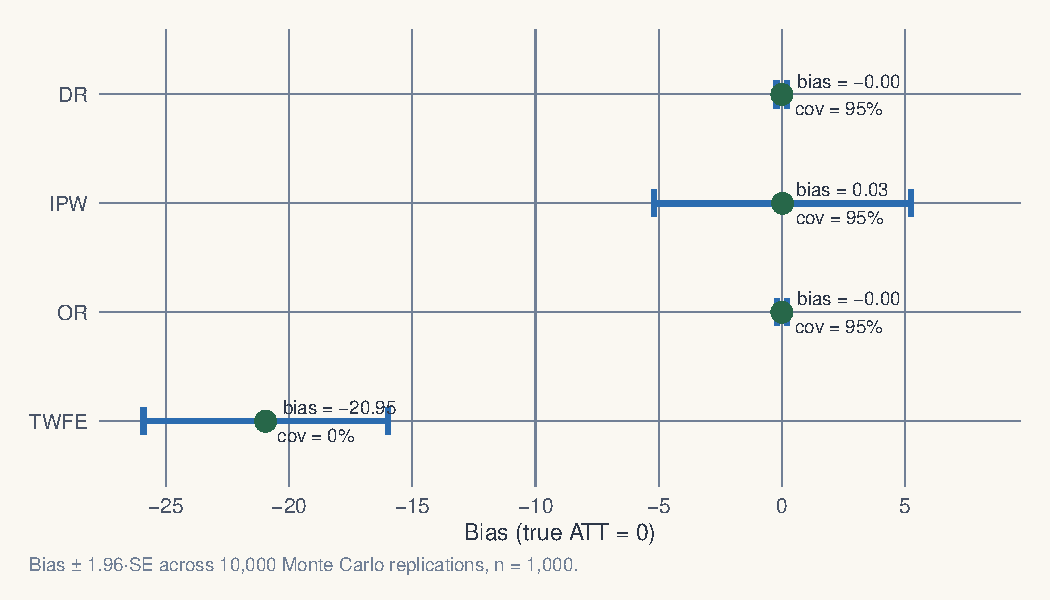
\includegraphics[width=0.68\textwidth]{figures/mc_dr_1.pdf}
\end{center}
\vspace{-0.2em}
\begin{center}
\small\color{warmgray}\itshape
When both models are correct, OR and DR concentrate tightly on the truth. IPW is unbiased but noisy. TWFE is off the map.
\end{center}
\end{frame}

%% ---------- L5-MC4: DGP4 results ----------
\begin{frame}{DGP 4 --- both models \textit{wrong}}
\vspace{0.4em}
\begin{center}
\small
\renewcommand{\arraystretch}{1.3}
\begin{tabular}{@{}lrrrrr@{}}
\toprule
            & \textbf{Bias} & \textbf{RMSE} & \textbf{SE} & \textbf{Coverage} & \textbf{CI length} \\
\midrule
TWFE        & $-16.38$ & $16.54$ & $3.63$ & $0.000$ & $14.22$ \\
OR          & $-5.20$  & $5.36$  & $1.29$ & $0.015$ & $5.05$  \\
\rowcolor{remixgreenlight}
IPW         & $-1.08$  & $2.66$  & $2.37$ & $0.949$ & $9.31$  \\
DR          & $-3.19$  & $3.45$  & $1.29$ & $0.308$ & $5.07$  \\
\bottomrule
\end{tabular}
\end{center}
\vspace{0.3em}
\begin{center}
\small\color{warmgray}\itshape
DR is \textit{not} magic. When both models fail, DR is biased and undercovers (0.31 vs.\ nominal 0.95). \;IPW alone now wins on coverage --- it doesn't rely on the outcome model.
\end{center}
\end{frame}

%% ---------- L5-MC5: DGP4 visualization ----------
\begin{frame}{DGP 4 --- the sampling distribution tells the same story}
\vspace{0.3em}
\begin{center}
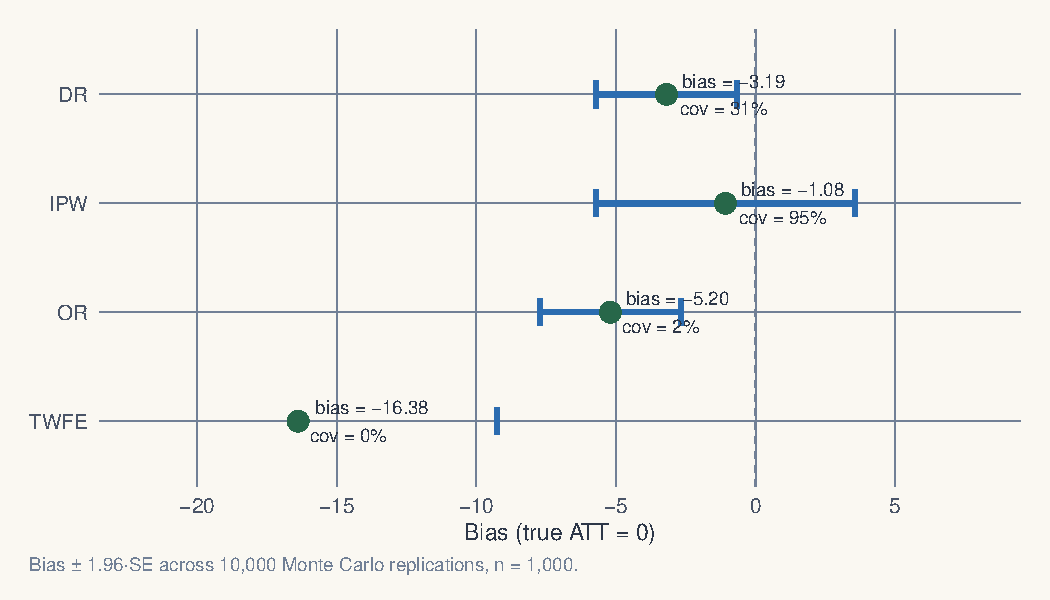
\includegraphics[width=0.68\textwidth]{figures/mc_dr_2.pdf}
\end{center}
\vspace{-0.2em}
\begin{center}
\small\color{warmgray}\itshape
DR no longer hugs the truth. IPW is wider but \textit{centered}. \;Doubly robust $\neq$ doubly unbeatable.
\end{center}
\end{frame}

%% ---------- L5-MC6: takeaway ----------
\begin{frame}{What the Monte Carlo teaches}
\vspace{0.4em}
\begin{itemize}\small
  \item \textbf{TWFE with additive $X$:} never wins. \;Coverage is zero in every DGP. \highlight{Stop using it as a default.}
  \item \textbf{OR:} efficient when the outcome model is right. Disaster when it's wrong (Bias $-5$, coverage $1.5\%$).
  \item \textbf{IPW:} less efficient but \textit{robust to outcome misspecification}. The unsexy workhorse.
  \item \textbf{DR:} best of both \textit{when at least one is right}. \;Not better than IPW when \textit{both} are wrong.
\end{itemize}
\vspace{0.4em}
\begin{center}
\small\color{warmgray}\itshape
``Doubly robust'' means \textit{robust to one misspecification.} \;Not two. \;Not magic.
\end{center}
\meta{Replication: \texttt{simulations/covariates/covariates\_monte\_carlo.\{do,R\}}; figures \texttt{mc\_dr\_1.png, mc\_dr\_2.png}.}
\end{frame}


%% =========================================================================
%% ABSORBED (was Section 3 'The Trap'): closing addendum to DR-DiD.
%% Pedagogy: DR is sometimes misdescribed as 'regression-with-pscore-as-
%% control'. That IS the trap, and it is exactly what DR is NOT.
%% =========================================================================


%% ---------- L3-Trap0: bridge — DR vs the misunderstanding ----------
\begin{frame}{Closing addendum: DR is \textit{not} regression-plus-pscore}
\footnotesize
A common misdescription you'll hear:
\vspace{0.3em}
\pullquote{Doubly robust DiD is just outcome regression plus the propensity score as another control.}{Heard at more than one seminar}

\vspace{0.6em}
\textbf{No.} \;That description conflates three different things:
\begin{itemize}\setlength\itemsep{2pt}
  \item what \textbf{outcome regression} actually does (model $\mu_0(X)$ on controls; impute counterfactuals),
  \item what \textbf{IPW} actually does (use $\widehat{p}(X)$ as a \textit{weight}, not a regressor),
  \item what \textbf{DR} actually does (combine the two).
\end{itemize}

\vspace{0.4em}
\highlight{Adding $\widehat{p}(X)$ as a regressor on the right-hand side is its own --- different --- estimator.} \;It's a trap. \;The next few slides walk through exactly why.
\end{frame}

%% ---------- L4-F1: the temptation ----------
\begin{frame}{A natural temptation}
\vspace{0.6em}
\pullquote{If the propensity score is the one-scalar summary of confounding, why not just add it as a regressor? Done.}{The audience, right now}
\vspace{0.6em}
\begin{itemize}\small
  \item It sounds right. Rosenbaum-Rubin says \textit{one scalar suffices}. Regression handles scalars.
  \item So: $\;\; Y_i \;=\; \alpha \;+\; \delta D_i \;+\; \gamma\, \widehat{p}(X_i) \;+\; \varepsilon_i$
  \item Surely this recovers $\delta$ as the ATT? \highlight{No.} And the reason matters.
\end{itemize}
\end{frame}

%% ---------- L4-F2: what's wrong with it ----------
\begin{frame}{What that regression actually assumes}
\vspace{0.4em}
\[
Y_i \;=\; \alpha \;+\; \delta D_i \;+\; \gamma\, \widehat{p}(X_i) \;+\; \varepsilon_i
\]
\vspace{0.1em}
\begin{itemize}\small
  \item No $D \times X$ interaction. No $D \times \widehat{p}$ interaction. \\
  \highlight{The treatment effect is forced constant} across the entire range of $\widehat{p}(X)$.
  \item Equivalently: the same dose of policy produces the same effect on a person with $\widehat{p}(X)=0.10$ as on a person with $\widehat{p}(X)=0.90$.
  \item That's an assumption about \highlight{the outcome side} --- one that Rosenbaum-Rubin says nothing about.
  \item Rosenbaum-Rubin gives you a valid \textit{reweighting} tool. It does not authorize regression-on-pscore.
\end{itemize}
\end{frame}

%% ---------- L4-F3: simulation ----------
\begin{frame}{A simulation makes it visible}
\vspace{-0.2em}
\begin{center}
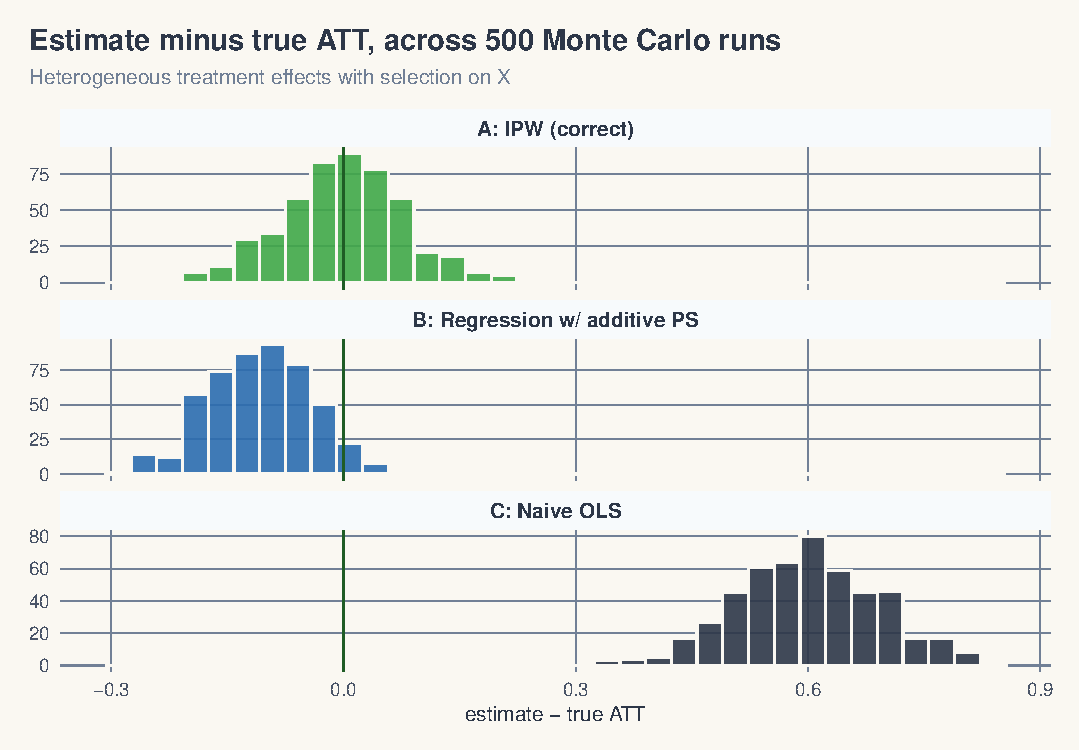
\includegraphics[width=0.80\linewidth,height=0.62\textheight,keepaspectratio]{figures/ipw_comparison.pdf}
\end{center}
\vspace{-0.4em}
\begin{center}
\footnotesize\color{warmgray}\itshape
500 reps. Heterogeneous $\delta(X) = 1 + 0.5\, X_1$.\;
Method A (IPW reweighting): bias $\approx 0$. \;
Method B (regression with $\widehat{p}$): \highlight{bias $\approx -10\%$}.
\end{center}
\meta{Code: \texttt{glasgow/decks/code/IPW-Demo/ipw\_simulation.R}.}
\end{frame}

%% ---------- L4-F4: codeblock ----------
\begin{frame}[fragile]{The simulation, one screen of R}
\vspace{0.1em}
\begin{lstlisting}[language=R,basicstyle=\ttfamily\scriptsize]
N  <- 1000
X1 <- rnorm(N); X2 <- rnorm(N)
p  <- plogis(0.5*X1 + 0.3*X2 - 0.2)        # true propensity
D  <- rbinom(N, 1, p)
Y0 <- X1 + 0.5*X2 + rnorm(N)
Y1 <- Y0 + (1 + 0.5*X1)                    # heterogeneous tau(X)
Y  <- D*Y1 + (1-D)*Y0

phat <- glm(D ~ X1 + X2, family=binomial)$fitted.values

# Method A: IPW -- reweight controls
w  <- ifelse(D==1, 1, phat/(1-phat))
A  <- mean(Y[D==1]) - weighted.mean(Y[D==0], w[D==0])

# Method B: regression with pscore as a control
B  <- coef(lm(Y ~ D + phat))["D"]          # <-- the trap
\end{lstlisting}
\meta{Full simulation: \texttt{decks/code/IPW-Demo/ipw\_simulation.R}}
\end{frame}

%% ---------- L4-F5: the intuition ----------
\begin{frame}{Weight versus regressor --- different uses of the same scalar}
\vspace{0.4em}
\begin{itemize}
  \item The propensity score is a \highlight{tool}. The same scalar can be used as:
  \begin{itemize}\small
    \item[--] a \textbf{weight} (Method A: reweight controls) --- recovers ATT
    \item[--] a \textbf{regressor} (Method B: add as control) --- imposes homogeneous effects
  \end{itemize}
  \item Same number. Different uses. \textit{Different identifying assumptions.}
  \item Method B's bias is not noise. It is the heterogeneity in $\delta(X)$ that the regression cannot see.
\end{itemize}
\vspace{0.5em}
\begin{block}{The lesson before DR}
\small
``Doubly robust'' is sometimes mis-summarized as ``IPW plus a regression control.'' \\[0.2em]
\highlight{That's wrong.} DR is something else --- it uses the pscore as a weight, AND it uses an outcome model. \\
But it does NOT use the pscore as a regressor.
\end{block}
\end{frame}

%% ---------- L4-F6: name the disease ----------
\begin{frame}{Name the disease: \textit{additive-control-side bias}}
\vspace{0.4em}
Whenever you put a covariate on the right-hand side of an outcome regression \textit{additively} (no $D \times X$ interaction), you force:
\vspace{-0.2em}
\[
\delta \;\;\text{is constant across all values of that covariate.}
\]
\vspace{-0.4em}
\begin{itemize}\small
  \item Method B (Lesson 4): the covariate is $\widehat{p}(X)$ --- a scalar summary of $X$. \\
        Force constant $\delta$ across $\widehat{p}(X)$. Heterogeneity in $\delta(X)$ is invisible.
  \item TWFE-with-controls (Lesson 2): the covariate is $X$ itself. \\
        Force constant $\delta$ across $X$. Heterogeneity in $\delta(X)$ is invisible.
  \item \highlight{Same disease, different costume.} Caetano \& Callaway (2024) name the TWFE version \textit{hidden linearity bias}. It's the same root.
\end{itemize}
\vspace{0.3em}
\begin{center}
\small\color{warmgray}\itshape
DR's escape: use $X$ and $\widehat{p}(X)$ as \textit{weights} and to model the \textit{counterfactual} $\mu_0(X)$ on controls only --- never as additive regressors of $Y$.
\end{center}
\end{frame}

%% =====================================================================
%%                                LESSON 4
%%        Caetano & Callaway: hidden linearity bias (same disease as L4)
%% =====================================================================
\remixsection{4.\ Hidden Linearity Bias \\[0.3em] {\normalsize\normalfont Caetano \& Callaway 2024}}

%% ---------- L6-F0: TWFE-with-controls has TWO distinct problems ----------
\begin{frame}{TWFE-with-controls has two distinct problems}
\vspace{0.4em}
The workhorse specification $Y_{it} = \alpha_i + \gamma_t + \delta D_{it} + X_{it}'\beta + \varepsilon_{it}$ is biased for two \textit{separate} reasons:
\vspace{0.5em}
\begin{enumerate}
  \item \highlight{The FE transformation throws away what you wanted to control for.} \\[0.2em]
  First-differencing $X_{it}$ leaves only $\Delta X$. The \textit{level} of $X$ is gone. Time-invariant $Z$ is gone entirely. \;\; (Caetano-Callaway 2024 --- this lesson.)
  \item \highlight{What's left enters additively, forcing constant $\delta$.} \\[0.2em]
  Whatever covariate survives the FE transformation sits on the RHS as an additive regressor with no $D{\times}X$ interaction. Same disease as Method B (Lesson 4).
\end{enumerate}
\vspace{0.5em}
\begin{center}
\small\color{warmgray}\itshape
This lesson covers problem (1). Problem (2) is the L4 callback we'll close on.
\end{center}
\end{frame}

%% ---------- L6-F1: the applied problem ----------
\begin{frame}{An applied problem you've already run}
\vspace{0.5em}
\pullquote{TWFE with time-varying controls is the workhorse DiD specification. Almost every DiD paper runs it.}{Anybody who's seen a job-market paper}
\vspace{0.5em}
\begin{itemize}
  \item Standard recipe: include population, income, demographic shares, region indicators, etc. on the right-hand side. Run TWFE. Done.
  \item \highlight{What if I told you that regression doesn't control for what you think it controls for?}
  \item Caetano \& Callaway (2024, R\&R \textit{REStat}): yes. The fixed-effect transformation quietly drops your $X$ levels and your time-invariant $Z$.
\end{itemize}
\end{frame}

%% ---------- L6-F2: the application — SYG laws ----------
\begin{frame}{An application: stand-your-ground laws (Cheng \& Hoekstra 2013)}
\vspace{0.5em}
\begin{itemize}\small
  \item 50 states, 2000--2010. 20 states adopt stand-your-ground laws. Outcome: log homicide rate.
  \item Treated states differ from controls in \highlight{levels}:
  \begin{itemize}\small
    \item[--] South dummy: std.\ diff. $= 0.81$  (large)
    \item[--] Poverty rate:  std.\ diff. $= 1.06$  (huge)
    \item[--] Median income: std.\ diff. $= -1.08$ (huge)
  \end{itemize}
  \item But the differences in \highlight{changes} of these covariates are small.
\end{itemize}
\vspace{0.6em}
\begin{block}{The headline result}
\small
TWFE with covariates: \;\;$\widehat{\alpha} = +0.067$, \;significant. \\
AIPW with the right covariates: \;$\widehat{\text{ATT}} \approx 0$, insignificant.\\[0.3em]
\highlight{The positive TWFE result is largely artefact of hidden linearity bias.}
\end{block}
\end{frame}

%% ---------- L6-F3: the intuition ----------
\begin{frame}{What TWFE actually controls for, after the FE transformation}
\vspace{0.4em}
You wrote down this model:
\vspace{-0.1em}
\[
Y_{it} \;=\; \alpha_i \;+\; \gamma_t \;+\; \delta D_{it} \;+\; X_{it}'\beta \;+\; Z_i'\eta \;+\; \varepsilon_{it}
\]
\vspace{0.1em}
First-difference (or within-transform) to kill $\alpha_i$:
\vspace{-0.2em}
\[
\Delta Y_{it} \;=\; \widetilde{\gamma}_t \;+\; \delta\, \Delta D_{it} \;+\; \Delta X_{it}'\beta \;+\; \Delta \varepsilon_{it}
\]
\vspace{0.1em}
\begin{itemize}\small
  \item $\alpha_i$ vanishes (good).
  \item $Z_i$ vanishes too (time-invariant). \highlight{Region: gone.}
  \item $X_{it}$ becomes $\Delta X_{it}$. \highlight{Population level: gone. Only population growth remains.}
  \item Your ``controls'' are now \textit{changes} in $X$, not levels.
\end{itemize}
\end{frame}

%% ---------- L6-F4: what the correct model is ----------
\begin{frame}{What you should be controlling for}
\vspace{0.5em}
The correct first-differenced model for $\Delta Y(0)$ (Caetano-Callaway Eq.\ 4):
\vspace{-0.2em}
\[
\Delta Y_{it}(0) \;=\; \widetilde{\gamma}_t \;+\; \underbrace{Z_i'\widetilde{\delta}_t}_{\text{time-inv}}
                                         \;+\; \underbrace{\Delta X_{it}'\beta_t}_{\text{changes}}
                                         \;+\; \underbrace{X_{i,t-1}'\widetilde{\beta}_t}_{\text{level}}
                                         \;+\; \Delta\varepsilon_{it}
\]
\vspace{0.1em}
\begin{itemize}\small
  \item \textbf{Time-invariant} $Z$ (region) belongs on the right --- because trends differ by region.
  \item \textbf{Pre-period level} $X_{i,t-1}$ belongs on the right --- because the level of population predicts the trend in homicides.
  \item TWFE drops both. \highlight{Hidden linearity bias.}
\end{itemize}
\end{frame}

%% ---------- L6-F5: the callback to Lesson 4 ----------
\begin{frame}{The L4 callback: problem (2) is the additive-RHS disease}
\vspace{0.3em}
We've covered problem (1) above --- the FE transformation throws away levels. \\
Problem (2) is the L4 disease, present in TWFE-with-controls too.
\vspace{0.4em}
\begin{center}
\renewcommand{\arraystretch}{1.4}
\footnotesize
\begin{tabular}{@{}lll@{}}
\toprule
\textbf{Estimator} & \textbf{What goes on RHS additively} & \textbf{What gets forced constant} \\
\midrule
\rowcolor{remixgreenlight}
Method B (L4)             & $\widehat{p}(X)$ as control          & $\delta$ across $\widehat{p}(X)$ \\
\rowcolor{remixgreenlight}
TWFE-with-controls (L2, L6) & $\Delta X$ as control              & $\delta$ across $\Delta X$       \\
\rowcolor{remixgreenlight}
General formulation       & $W = f(X)$ as additive RHS regressor & $\delta$ across $W$              \\
\bottomrule
\end{tabular}
\end{center}
\vspace{0.3em}
\begin{itemize}\small
  \item Problem (1) is C\&C's contribution: \textit{what} you control for is wrong.
  \item Problem (2) is the L4 disease: \textit{how} you control for it is wrong.
  \item TWFE-with-controls catches both. DR escapes both --- using $X$ and $\widehat{p}(X)$ as \highlight{weights}, not as additive regressors.
\end{itemize}
\end{frame}

%% ---------- L6-F6: the fix — AIPW ----------
\begin{frame}{The fix: AIPW with $(X_{t-1},\, Z)$}
\vspace{0.5em}
Caetano-Callaway's recommended estimator:
\vspace{-0.1em}
\[
\widehat{\text{ATT}} \;=\; \widehat{\mathbb{E}}_{D=1}\!\big[\Delta Y \;-\; \widehat{m}_0(X_{t-1}, Z)\big]
\]
\vspace{0.1em}
\begin{itemize}\small
  \item $\widehat{m}_0(X_{t-1}, Z)$: outcome regression of $\Delta Y$ on \textit{pre-treatment level} of $X$ and \textit{time-invariant} $Z$ --- fit on \textbf{controls only}.
  \item \highlight{Why $X_{t-1}$, not $X_t$?} \;Because $X_t$ in the post-period could itself be affected by treatment. The pre-treatment level is uncontaminated.
  \item Combine with IPW on a generalized propensity score (same conditioning set) for full doubly-robust safety.
  \item CC's fully preferred spec also includes $\Delta X = X_t - X_{t-1}$ for dimension reduction. R: \texttt{pte}, \texttt{twfeweights}.
\end{itemize}
\end{frame}

%% ---------- L6-F6a: A student asks — why X_{t-1}, not X_t? ----------
\begin{frame}{Pre-treatment $X$ is uncontaminated --- post-treatment $X$ is not}
\vspace{0.4em}
\pullquote{Why $X_{t-1}$ and not $X_t$? You're throwing away the most recent data point.}{A student, raising a hand}
\vspace{0.4em}
\begin{itemize}\small
  \item $X_t$ sits \highlight{downstream of treatment}. If the policy moves $X$ --- even a little --- you've controlled for a \textit{post-treatment outcome}.
  \item Conditioning on a post-treatment variable doesn't reduce bias. It \highlight{re-introduces} bias --- the bad-controls problem (Angrist--Pischke 2009, Ch.\ 3).
  \item $X_{t-1}$ is settled before $D$ is assigned. It carries the selection information without carrying any of the treatment.
\end{itemize}
\vspace{0.3em}
\begin{center}
\small\color{warmgray}\itshape
The rule generalizes: \;condition on the latest pre-treatment value, never the contemporaneous one.
\end{center}
\meta{Caetano \& Callaway (2024), \S 3; classic ``bad controls'' point goes back to Rosenbaum (1984).}
\end{frame}

%% ---------- L6-F7: SYG numbers ----------
\begin{frame}{Stand-your-ground revisited --- the numbers}
\vspace{0.5em}
\begin{center}
\renewcommand{\arraystretch}{1.4}
\footnotesize
\begin{tabular}{@{}lcc@{}}
\toprule
\textbf{Specification}                                & \textbf{$\widehat{\text{ATT}}$} & \textbf{SE} \\
\midrule
TWFE with $\Delta X$ (the standard recipe)            & $+0.067$               & 0.026       \\
Reg.\ adj.\ with $\Delta X + Z$                        & $+0.106$               & 0.058       \\
\rowcolor{remixgreenlight}
Reg.\ adj.\ with $X_{t-1} + Z$ \;(\textit{Caetano-Callaway preferred}) & $+0.019$ & 0.043 \\
Reg.\ adj.\ with $\Delta X + X_{t-1} + Z$              & $+0.078$               & 0.180       \\
\bottomrule
\end{tabular}
\end{center}
\vspace{0.6em}
\begin{itemize}\small
  \item The TWFE positive effect ($+6.7\%$) shrinks to near-zero ($+1.9\%$) when you control for \textit{levels} of $X$ and $Z$.
  \item The bias was hidden in plain sight --- the regression compiled fine. It just wasn't controlling for what we thought.
\end{itemize}
\end{frame}


%% =====================================================================
%%                                LESSON 5
%% =====================================================================
\remixsection{5.\ Choosing \& checking $X$ \\[0.3em] {\normalsize\normalfont The practical close --- picking, balance, and when controls are unnecessary}}

%% ---------- L8-F1: picking covariates ----------
\begin{frame}{Picking $X$: theory or LASSO on $\Delta Y(0)$}
You want $X$ that (i) predicts the treatment \textit{and} (ii) predicts the untreated trend. \;\highlight{Pre-treatment only} --- post-treatment $X$ can be affected by $D$ and will leak.

\vspace{0.4em}
\textbf{Two paths to choose which $X$:}
\begin{itemize}\small
  \item \textbf{Theory / common sense.} \;Variables you believe drive both selection and the untreated trend. \;This is how most of it actually gets done.
  \item \textbf{Data-driven.} \;LASSO (or another selector) on
  \begin{center}\footnotesize
  $\Delta Y(0)_i \;\sim\; X_i, \quad$ fit on untreated unit-periods only.
  \end{center}
  Keep what LASSO keeps.
\end{itemize}

\vspace{0.4em}
\textbf{The regressand is \boldmath$\Delta Y(0)$.} \;Not $Y(1)$. Not post-treatment $Y$ --- that's $Y(1)$, and using it lets $D$ leak through the back door. This is \highlight{Heckman-Ichimura-Todd (1997)} logic: the data can only teach you which $X$'s predict the untreated counterfactual trend.

\vspace{0.3em}
Beyond that --- functional form, interactions, transformations --- the data is mostly silent.
\end{frame}

%% ---------- L8-F2a: balanced — the easy case ----------
\begin{frame}{If $X$ is balanced, you don't need to control for it}
\vspace{0.4em}
Same logic as an RCT: \;balanced $X$ across treatment and control makes the comparison fair without conditioning.

\vspace{0.7em}
\textbf{Worked example.} \;Let sex be the only confounder. Within sex, the untreated trends are:
\vspace{0.4em}
\begin{center}
$\Delta Y^0_{\text{men}} \;=\; 10 - 6 \;=\; 4 \qquad\qquad \Delta Y^0_{\text{women}} \;=\; 8 - 5 \;=\; 3.$
\end{center}

\vspace{0.7em}
\textbf{Balanced --- both groups 50\% male.}
\vspace{0.2em}
\begin{center}
$\mathbb{E}[\Delta Y^0 \mid D{=}1] \;=\; 0.5(4) + 0.5(3) \;=\; 3.5 \;=\; \mathbb{E}[\Delta Y^0 \mid D{=}0].$
\end{center}

\vspace{0.5em}
\highlight{Unconditional PT holds.} \;You didn't condition on sex --- and you didn't need to.
\end{frame}

%% ---------- L8-F2b: imbalanced — the bias appears ----------
\begin{frame}{Imbalance turns a confounder into bias}
\vspace{0.4em}
Same untreated trends as before --- men $+4$, women $+3$ --- but now the groups have different sex composition:

\vspace{0.7em}
\textbf{Imbalanced --- treated 75\% male, control 25\% male.}
\vspace{0.3em}
\begin{center}
$\mathbb{E}[\Delta Y^0 \mid D{=}1] \;=\; 0.75(4) + 0.25(3) \;=\; 3.75$ \\[0.4em]
$\mathbb{E}[\Delta Y^0 \mid D{=}0] \;=\; 0.25(4) + 0.75(3) \;=\; 3.25.$
\end{center}

\vspace{0.6em}
\highlight{Gap $=$ 0.5.} \;That's the bias a naive DiD on $\Delta Y$ would carry.

\vspace{0.6em}
\textbf{Takeaway.} \;Balance is what licenses unconditional PT. \;Imbalance turns a $Y^0$-predictor into a bias on $\Delta Y^0$.
\end{frame}

%% ---------- L8-F3: balance — normalized differences ----------
\begin{frame}{Check the balance: normalized differences}
\vspace{0.6em}
Before you trust your $X$, check that the treated and control groups are \textit{actually} comparable on it.
\vspace{0.6em}
\begin{block}{Normalized difference}
\centering
\large
$\text{Norm. Diff}_{X} \;=\; \dfrac{\overline{X}_T - \overline{X}_C}{\sqrt{(S^2_T + S^2_C)/2}}$
\end{block}
\vspace{0.6em}
\begin{itemize}\small
  \item A unit-free imbalance measure --- comparable across variables.
  \item \highlight{Rule of thumb: $< 0.25$.} \;Above that, classical OLS/IPW have trouble.
  \item Unlike a $t$-statistic, it doesn't shrink to zero just because the sample is small.
\end{itemize}
\meta{Imbens \& Rubin (2015), \textit{Causal Inference for Statistics, Social, and Biomedical Sciences}, Ch.\ 14.}
\end{frame}

%% ---------- L8-F4a: balance — the two jobs of a confounder ----------
\begin{frame}{What balance tells you (and what it doesn't)}
\vspace{0.5em}
A confounder has \textit{two} jobs:
\vspace{0.5em}
\begin{enumerate}
  \item $X \to D$: \;different distribution in treated vs.\ control.
  \item $X \to \Delta\mathbb{E}[Y^0]$: \;predicts the untreated outcome trend.
\end{enumerate}
\vspace{0.6em}
\highlight{The balance check only diagnoses (1).}
\vspace{0.5em}
\begin{itemize}\small
  \item Pick $X$ theoretically --- variables you believe predict $Y^0$ trends.
  \item \textit{Then} run normalized differences to see whether they're differentially distributed.
  \item Imbalance + predictiveness $\Rightarrow$ controlling matters. \;Imbalance without predictiveness $\Rightarrow$ noise.
\end{itemize}
\end{frame}

%% ---------- L8-F4b: don't over-spend on already-balanced X ----------
\begin{frame}{Don't over-spend on already-balanced $X$}
\vspace{0.5em}
Adding controls in OLS DiD is cheap. \;In IPW or DR, it isn't.

\vspace{0.6em}
The propensity score is fit by logistic regression, which is fragile in high dimensions:

\vspace{0.5em}
\begin{block}{Events-per-variable rule}
\centering
Roughly \highlight{5--10 events per covariate} for stable logistic estimates, \\ where ``events'' $=$ treated units.
\end{block}

\vspace{0.6em}
\textbf{Implication.} \;A balanced $X$ that doesn't strongly predict $\Delta Y^0$ doesn't deserve a slot in the pscore model. \;The balance table tells you where to spend the budget.
\meta{EPV guideline: Peduzzi et al.\ (1996), \textit{J.\ Clin.\ Epidemiol.}}
\end{frame}

%% ---------- L8-F5: a real balance table ----------
\begin{frame}{A balance table in the wild}
\vspace{0.3em}
\begin{center}
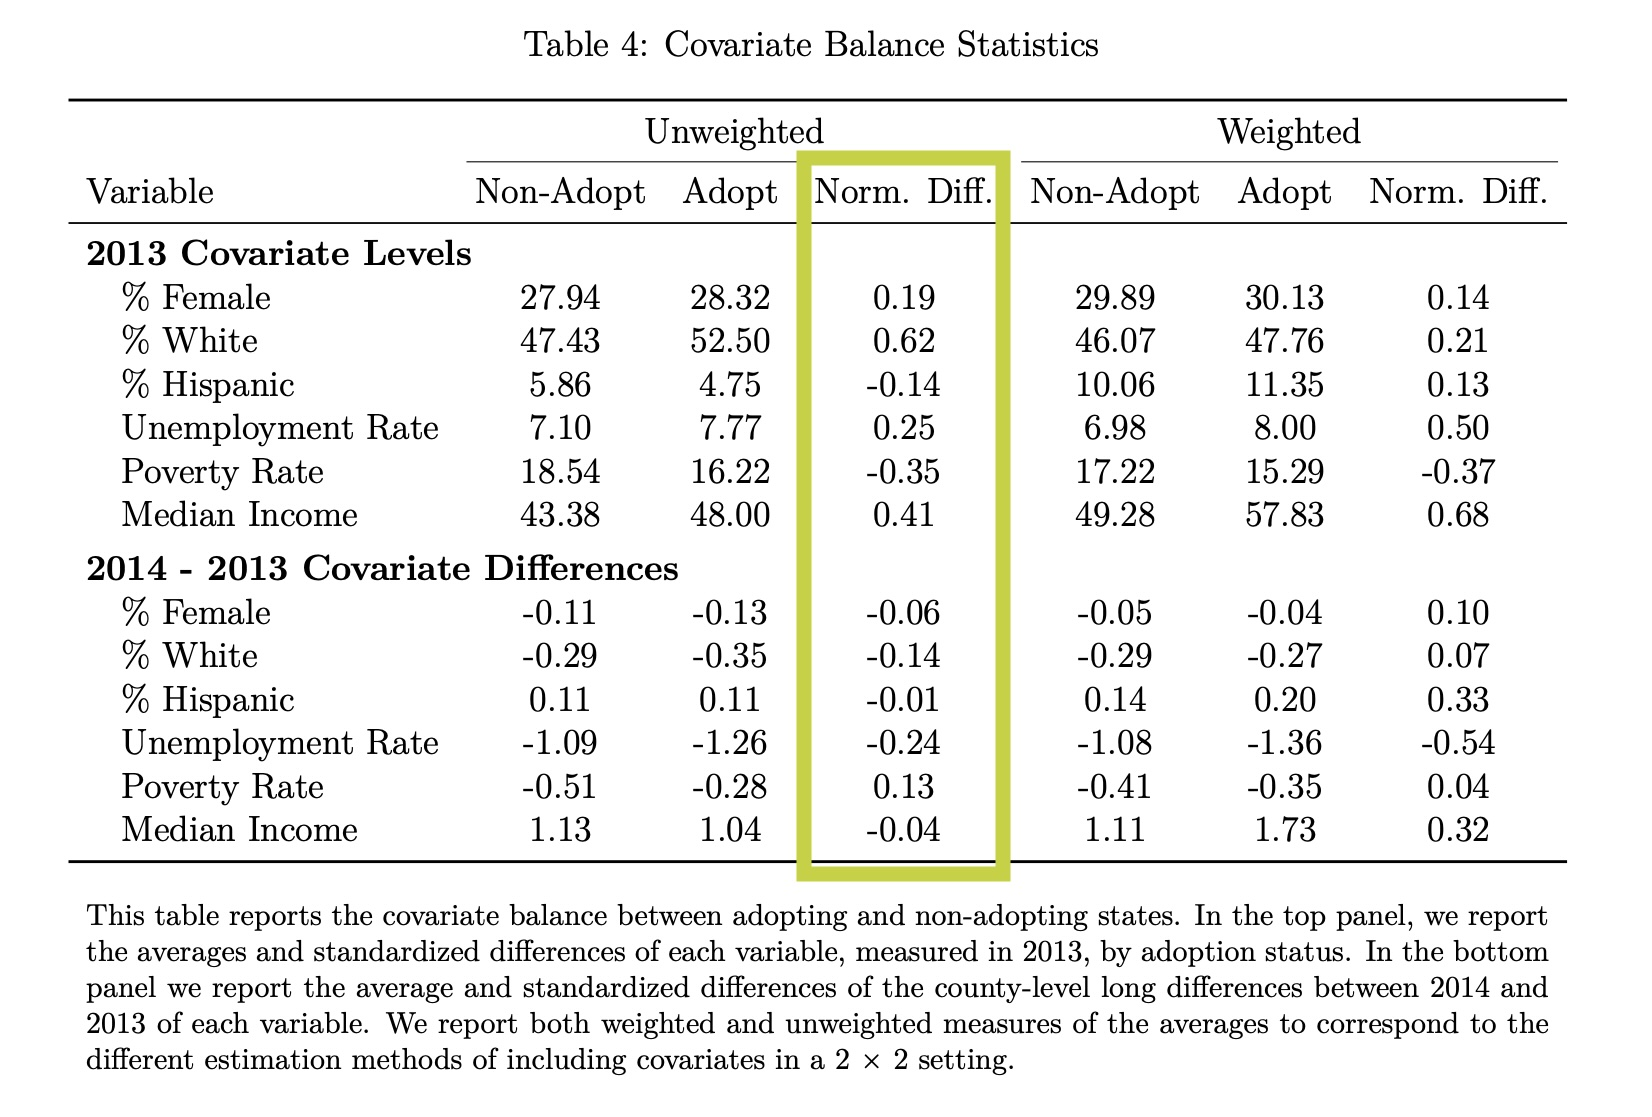
\includegraphics[width=0.74\textwidth,height=0.68\textheight,keepaspectratio]{figures/table_jel_covariates.jpg}
\end{center}
\vspace{0.1em}
\begin{center}
\scriptsize\color{warmgray}\itshape
Every variable, its treated mean, its control mean, the normalized difference. \;One column tells you whether the design will make you sweat.
\end{center}
\end{frame}

%% ---------- Recap ----------
\begin{frame}{What we've done this afternoon}
\vspace{0.3em}
\begin{enumerate}\small
  \item Conditional PT --- the new identifying assumption
  \item Outcome regression: model the trend, impute the counterfactual
  \item IPW: reweight controls to look like the treated
  \item Doubly robust: pscore as a \textit{weight} (not regressor) + outcome model --- and why \textit{controlling for} the pscore is the trap
  \item Hidden linearity bias (Caetano-Callaway): \textit{same disease}, costume = TWFE-with-controls
\end{enumerate}
\vspace{0.5em}
\begin{center}
\small\color{warmgray}\itshape
The unifying lesson: covariates on the additive RHS of an outcome regression impose constraints on $\delta$. \\
DR's escape is to use them as \highlight{weights}, not regressors.
\end{center}
\end{frame}

%% ---------- Tomorrow preview ----------
\begin{frame}{Tomorrow}
\vspace{0.4em}
\begin{itemize}
  \item \textbf{Day 3:} when even covariates can't save you. Synthetic control, the frontier methods.
  \item Plus: when treatment timing differs across units --- the staggered-adoption mess (Goodman-Bacon, Callaway-Sant'Anna, Sun-Abraham, BJS, dCdH).
\end{itemize}
\end{frame}

%% ---------- Closing one-sentence linger ----------
\begin{frame}[plain]
\begin{tikzpicture}[remember picture,overlay]
\fill[cream] (current page.south west) rectangle (current page.north east);
\node[anchor=center, text width=0.84\paperwidth, align=center, text=charcoal] at (current page.center) {%
  \fontsize{18pt}{26pt}\selectfont
  Use the pscore as a {\color{accent}\bfseries weight,}\\[0.3em]
  not as a {\color{accent}\bfseries regressor.}\\[0.6em]
  That is the difference between {\color{accent}\bfseries doubly robust}\\[0.2em]
  and {\color{accent}\bfseries doubly biased.}
};
\draw[accent, line width=1pt] ([yshift=1.4cm,xshift=0.25\paperwidth]current page.south west) -- ([yshift=1.4cm,xshift=-0.25\paperwidth]current page.south east);
\end{tikzpicture}
\end{frame}

\end{document}
